% Created by tikzDevice version 0.12.3.1 on 2023-05-30 21:55:45
% !TEX encoding = UTF-8 Unicode
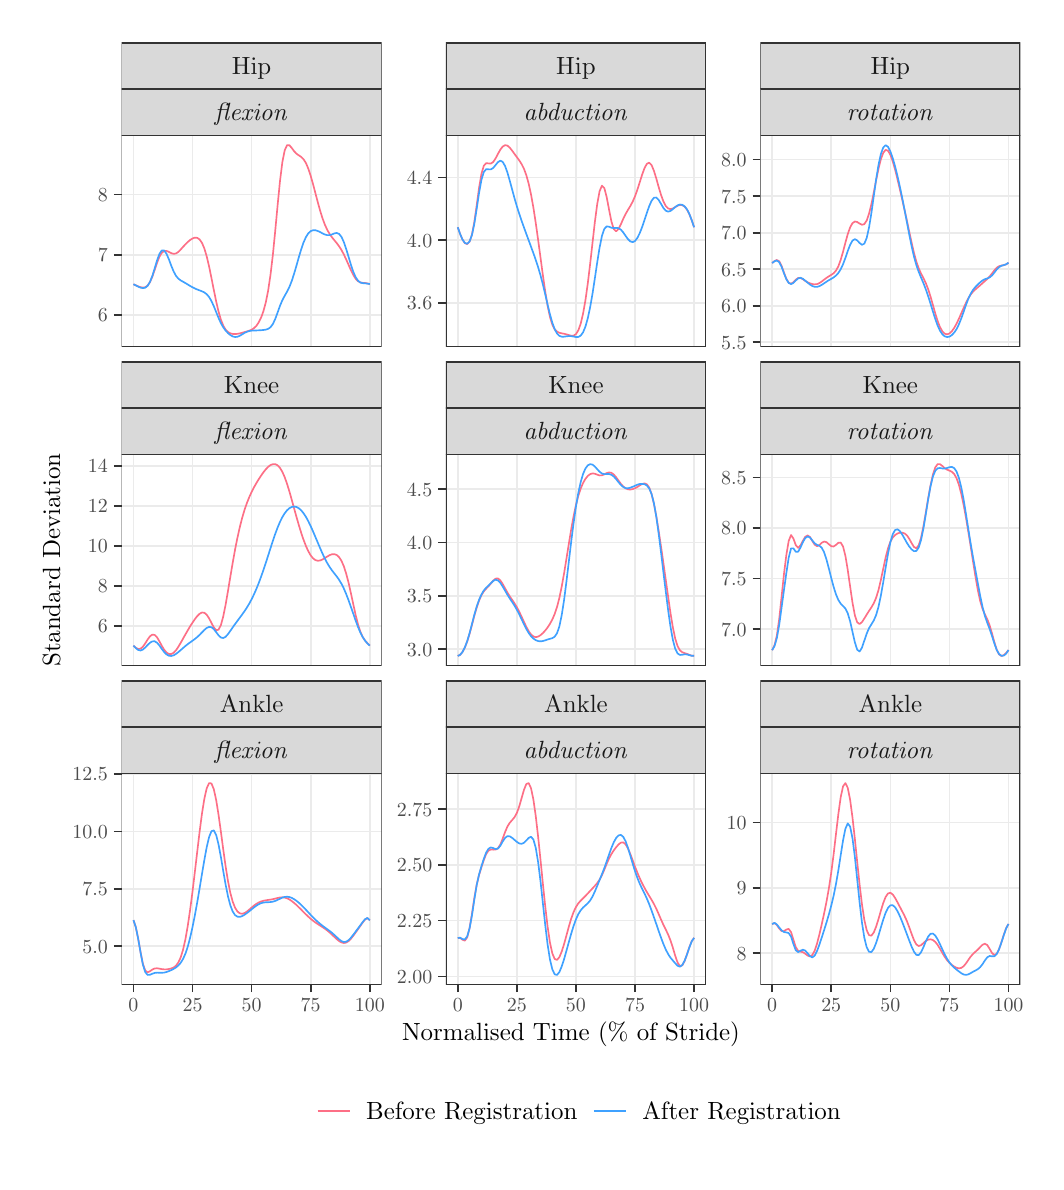
\begin{tikzpicture}[x=1pt,y=1pt]
\definecolor{fillColor}{RGB}{255,255,255}
\path[use as bounding box,fill=fillColor,fill opacity=0.00] (0,0) rectangle (364.19,409.72);
\begin{scope}
\path[clip] (  0.00,  0.00) rectangle (364.19,409.72);
\definecolor{drawColor}{RGB}{255,255,255}
\definecolor{fillColor}{RGB}{255,255,255}

\path[draw=drawColor,line width= 0.6pt,line join=round,line cap=round,fill=fillColor] (  0.00,  0.00) rectangle (364.19,409.72);
\end{scope}
\begin{scope}
\path[clip] ( 33.94,294.47) rectangle (127.90,370.72);
\definecolor{fillColor}{RGB}{255,255,255}

\path[fill=fillColor] ( 33.94,294.47) rectangle (127.90,370.72);
\definecolor{drawColor}{gray}{0.92}

\path[draw=drawColor,line width= 0.6pt,line join=round] ( 33.94,305.89) --
	(127.90,305.89);

\path[draw=drawColor,line width= 0.6pt,line join=round] ( 33.94,327.66) --
	(127.90,327.66);

\path[draw=drawColor,line width= 0.6pt,line join=round] ( 33.94,349.42) --
	(127.90,349.42);

\path[draw=drawColor,line width= 0.6pt,line join=round] ( 38.22,294.47) --
	( 38.22,370.72);

\path[draw=drawColor,line width= 0.6pt,line join=round] ( 59.57,294.47) --
	( 59.57,370.72);

\path[draw=drawColor,line width= 0.6pt,line join=round] ( 80.92,294.47) --
	( 80.92,370.72);

\path[draw=drawColor,line width= 0.6pt,line join=round] (102.27,294.47) --
	(102.27,370.72);

\path[draw=drawColor,line width= 0.6pt,line join=round] (123.63,294.47) --
	(123.63,370.72);
\definecolor{drawColor}{RGB}{253,111,134}

\path[draw=drawColor,line width= 0.6pt,line join=round] ( 38.22,317.00) --
	( 39.07,316.62) --
	( 39.92,316.24) --
	( 40.78,315.94) --
	( 41.63,315.79) --
	( 42.49,315.93) --
	( 43.34,316.53) --
	( 44.19,317.78) --
	( 45.05,319.74) --
	( 45.90,322.22) --
	( 46.76,324.78) --
	( 47.61,326.94) --
	( 48.46,328.37) --
	( 49.32,329.04) --
	( 50.17,329.06) --
	( 51.03,328.69) --
	( 51.88,328.23) --
	( 52.74,327.98) --
	( 53.59,328.12) --
	( 54.44,328.70) --
	( 55.30,329.56) --
	( 56.15,330.52) --
	( 57.01,331.44) --
	( 57.86,332.28) --
	( 58.71,333.00) --
	( 59.57,333.55) --
	( 60.42,333.84) --
	( 61.28,333.76) --
	( 62.13,333.18) --
	( 62.98,331.96) --
	( 63.84,329.94) --
	( 64.69,327.08) --
	( 65.55,323.45) --
	( 66.40,319.30) --
	( 67.26,314.97) --
	( 68.11,310.81) --
	( 68.96,307.16) --
	( 69.82,304.21) --
	( 70.67,302.05) --
	( 71.53,300.61) --
	( 72.38,299.74) --
	( 73.23,299.27) --
	( 74.09,299.05) --
	( 74.94,299.00) --
	( 75.80,299.08) --
	( 76.65,299.25) --
	( 77.50,299.47) --
	( 78.36,299.72) --
	( 79.21,299.96) --
	( 80.07,300.22) --
	( 80.92,300.58) --
	( 81.77,301.13) --
	( 82.63,301.97) --
	( 83.48,303.20) --
	( 84.34,304.92) --
	( 85.19,307.28) --
	( 86.05,310.47) --
	( 86.90,314.77) --
	( 87.75,320.46) --
	( 88.61,327.74) --
	( 89.46,336.37) --
	( 90.32,345.61) --
	( 91.17,354.24) --
	( 92.02,361.07) --
	( 92.88,365.41) --
	( 93.73,367.26) --
	( 94.59,367.22) --
	( 95.44,366.22) --
	( 96.29,365.06) --
	( 97.15,364.16) --
	( 98.00,363.56) --
	( 98.86,363.00) --
	( 99.71,362.15) --
	(100.57,360.76) --
	(101.42,358.74) --
	(102.27,356.15) --
	(103.13,353.12) --
	(103.98,349.88) --
	(104.84,346.62) --
	(105.69,343.55) --
	(106.54,340.82) --
	(107.40,338.52) --
	(108.25,336.65) --
	(109.11,335.17) --
	(109.96,333.97) --
	(110.81,332.92) --
	(111.67,331.88) --
	(112.52,330.74) --
	(113.38,329.40) --
	(114.23,327.80) --
	(115.08,325.99) --
	(115.94,324.04) --
	(116.79,322.11) --
	(117.65,320.38) --
	(118.50,319.01) --
	(119.36,318.12) --
	(120.21,317.67) --
	(121.06,317.51) --
	(121.92,317.45) --
	(122.77,317.32) --
	(123.63,317.06);
\definecolor{drawColor}{RGB}{63,161,255}

\path[draw=drawColor,line width= 0.6pt,line join=round] ( 38.22,317.00) --
	( 39.07,316.58) --
	( 39.92,316.14) --
	( 40.78,315.78) --
	( 41.63,315.60) --
	( 42.49,315.76) --
	( 43.34,316.44) --
	( 44.19,317.83) --
	( 45.05,320.00) --
	( 45.90,322.78) --
	( 46.76,325.64) --
	( 47.61,327.95) --
	( 48.46,329.22) --
	( 49.32,329.21) --
	( 50.17,328.01) --
	( 51.03,326.01) --
	( 51.88,323.72) --
	( 52.74,321.63) --
	( 53.59,320.06) --
	( 54.44,319.04) --
	( 55.30,318.39) --
	( 56.15,317.91) --
	( 57.01,317.42) --
	( 57.86,316.91) --
	( 58.71,316.39) --
	( 59.57,315.90) --
	( 60.42,315.47) --
	( 61.28,315.10) --
	( 62.13,314.78) --
	( 62.98,314.45) --
	( 63.84,314.04) --
	( 64.69,313.40) --
	( 65.55,312.40) --
	( 66.40,310.95) --
	( 67.26,309.08) --
	( 68.11,306.96) --
	( 68.96,304.85) --
	( 69.82,302.97) --
	( 70.67,301.45) --
	( 71.53,300.27) --
	( 72.38,299.36) --
	( 73.23,298.65) --
	( 74.09,298.15) --
	( 74.94,297.93) --
	( 75.80,298.03) --
	( 76.65,298.39) --
	( 77.50,298.90) --
	( 78.36,299.42) --
	( 79.21,299.83) --
	( 80.07,300.09) --
	( 80.92,300.23) --
	( 81.77,300.29) --
	( 82.63,300.31) --
	( 83.48,300.35) --
	( 84.34,300.40) --
	( 85.19,300.48) --
	( 86.05,300.60) --
	( 86.90,300.88) --
	( 87.75,301.48) --
	( 88.61,302.64) --
	( 89.46,304.47) --
	( 90.32,306.81) --
	( 91.17,309.21) --
	( 92.02,311.23) --
	( 92.88,312.85) --
	( 93.73,314.33) --
	( 94.59,316.07) --
	( 95.44,318.24) --
	( 96.29,320.87) --
	( 97.15,323.81) --
	( 98.00,326.84) --
	( 98.86,329.70) --
	( 99.71,332.17) --
	(100.57,334.09) --
	(101.42,335.42) --
	(102.27,336.20) --
	(103.13,336.52) --
	(103.98,336.51) --
	(104.84,336.25) --
	(105.69,335.85) --
	(106.54,335.39) --
	(107.40,334.98) --
	(108.25,334.74) --
	(109.11,334.75) --
	(109.96,335.01) --
	(110.81,335.37) --
	(111.67,335.54) --
	(112.52,335.20) --
	(113.38,334.13) --
	(114.23,332.28) --
	(115.08,329.80) --
	(115.94,326.96) --
	(116.79,324.09) --
	(117.65,321.55) --
	(118.50,319.57) --
	(119.36,318.28) --
	(120.21,317.62) --
	(121.06,317.40) --
	(121.92,317.34) --
	(122.77,317.23) --
	(123.63,317.06);
\definecolor{drawColor}{gray}{0.20}

\path[draw=drawColor,line width= 0.6pt,line join=round,line cap=round] ( 33.94,294.47) rectangle (127.90,370.72);
\end{scope}
\begin{scope}
\path[clip] ( 33.94,179.21) rectangle (127.90,255.47);
\definecolor{fillColor}{RGB}{255,255,255}

\path[fill=fillColor] ( 33.94,179.21) rectangle (127.90,255.47);
\definecolor{drawColor}{gray}{0.92}

\path[draw=drawColor,line width= 0.6pt,line join=round] ( 33.94,193.54) --
	(127.90,193.54);

\path[draw=drawColor,line width= 0.6pt,line join=round] ( 33.94,208.01) --
	(127.90,208.01);

\path[draw=drawColor,line width= 0.6pt,line join=round] ( 33.94,222.47) --
	(127.90,222.47);

\path[draw=drawColor,line width= 0.6pt,line join=round] ( 33.94,236.94) --
	(127.90,236.94);

\path[draw=drawColor,line width= 0.6pt,line join=round] ( 33.94,251.41) --
	(127.90,251.41);

\path[draw=drawColor,line width= 0.6pt,line join=round] ( 38.22,179.21) --
	( 38.22,255.47);

\path[draw=drawColor,line width= 0.6pt,line join=round] ( 59.57,179.21) --
	( 59.57,255.47);

\path[draw=drawColor,line width= 0.6pt,line join=round] ( 80.92,179.21) --
	( 80.92,255.47);

\path[draw=drawColor,line width= 0.6pt,line join=round] (102.27,179.21) --
	(102.27,255.47);

\path[draw=drawColor,line width= 0.6pt,line join=round] (123.63,179.21) --
	(123.63,255.47);
\definecolor{drawColor}{RGB}{253,111,134}

\path[draw=drawColor,line width= 0.6pt,line join=round] ( 38.22,186.41) --
	( 39.07,185.66) --
	( 39.92,185.20) --
	( 40.78,185.30) --
	( 41.63,186.02) --
	( 42.49,187.25) --
	( 43.34,188.62) --
	( 44.19,189.78) --
	( 45.05,190.40) --
	( 45.90,190.28) --
	( 46.76,189.39) --
	( 47.61,187.97) --
	( 48.46,186.36) --
	( 49.32,184.94) --
	( 50.17,183.93) --
	( 51.03,183.40) --
	( 51.88,183.38) --
	( 52.74,183.84) --
	( 53.59,184.74) --
	( 54.44,185.99) --
	( 55.30,187.44) --
	( 56.15,188.96) --
	( 57.01,190.49) --
	( 57.86,191.98) --
	( 58.71,193.41) --
	( 59.57,194.75) --
	( 60.42,196.00) --
	( 61.28,197.09) --
	( 62.13,197.93) --
	( 62.98,198.38) --
	( 63.84,198.30) --
	( 64.69,197.59) --
	( 65.55,196.29) --
	( 66.40,194.63) --
	( 67.26,193.02) --
	( 68.11,192.01) --
	( 68.96,192.16) --
	( 69.82,193.83) --
	( 70.67,196.97) --
	( 71.53,201.24) --
	( 72.38,206.17) --
	( 73.23,211.32) --
	( 74.09,216.37) --
	( 74.94,221.11) --
	( 75.80,225.41) --
	( 76.65,229.23) --
	( 77.50,232.57) --
	( 78.36,235.46) --
	( 79.21,237.94) --
	( 80.07,240.08) --
	( 80.92,241.95) --
	( 81.77,243.61) --
	( 82.63,245.13) --
	( 83.48,246.54) --
	( 84.34,247.85) --
	( 85.19,249.06) --
	( 86.05,250.13) --
	( 86.90,251.02) --
	( 87.75,251.66) --
	( 88.61,252.00) --
	( 89.46,251.99) --
	( 90.32,251.56) --
	( 91.17,250.66) --
	( 92.02,249.23) --
	( 92.88,247.28) --
	( 93.73,244.86) --
	( 94.59,242.07) --
	( 95.44,239.05) --
	( 96.29,235.94) --
	( 97.15,232.86) --
	( 98.00,229.90) --
	( 98.86,227.13) --
	( 99.71,224.60) --
	(100.57,222.37) --
	(101.42,220.50) --
	(102.27,219.02) --
	(103.13,217.96) --
	(103.98,217.32) --
	(104.84,217.09) --
	(105.69,217.19) --
	(106.54,217.55) --
	(107.40,218.07) --
	(108.25,218.62) --
	(109.11,219.11) --
	(109.96,219.43) --
	(110.81,219.48) --
	(111.67,219.17) --
	(112.52,218.40) --
	(113.38,217.08) --
	(114.23,215.12) --
	(115.08,212.48) --
	(115.94,209.20) --
	(116.79,205.42) --
	(117.65,201.40) --
	(118.50,197.52) --
	(119.36,194.11) --
	(120.21,191.45) --
	(121.06,189.56) --
	(121.92,188.27) --
	(122.77,187.29) --
	(123.63,186.43);
\definecolor{drawColor}{RGB}{63,161,255}

\path[draw=drawColor,line width= 0.6pt,line join=round] ( 38.22,186.41) --
	( 39.07,185.53) --
	( 39.92,184.86) --
	( 40.78,184.66) --
	( 41.63,185.00) --
	( 42.49,185.75) --
	( 43.34,186.65) --
	( 44.19,187.46) --
	( 45.05,187.96) --
	( 45.90,187.99) --
	( 46.76,187.46) --
	( 47.61,186.46) --
	( 48.46,185.24) --
	( 49.32,184.10) --
	( 50.17,183.25) --
	( 51.03,182.77) --
	( 51.88,182.68) --
	( 52.74,182.92) --
	( 53.59,183.42) --
	( 54.44,184.07) --
	( 55.30,184.81) --
	( 56.15,185.56) --
	( 57.01,186.29) --
	( 57.86,186.97) --
	( 58.71,187.59) --
	( 59.57,188.20) --
	( 60.42,188.82) --
	( 61.28,189.52) --
	( 62.13,190.32) --
	( 62.98,191.20) --
	( 63.84,192.08) --
	( 64.69,192.81) --
	( 65.55,193.20) --
	( 66.40,193.07) --
	( 67.26,192.39) --
	( 68.11,191.31) --
	( 68.96,190.16) --
	( 69.82,189.35) --
	( 70.67,189.16) --
	( 71.53,189.62) --
	( 72.38,190.57) --
	( 73.23,191.76) --
	( 74.09,193.00) --
	( 74.94,194.21) --
	( 75.80,195.37) --
	( 76.65,196.51) --
	( 77.50,197.67) --
	( 78.36,198.88) --
	( 79.21,200.18) --
	( 80.07,201.60) --
	( 80.92,203.18) --
	( 81.77,204.94) --
	( 82.63,206.88) --
	( 83.48,209.01) --
	( 84.34,211.31) --
	( 85.19,213.76) --
	( 86.05,216.33) --
	( 86.90,218.98) --
	( 87.75,221.66) --
	( 88.61,224.29) --
	( 89.46,226.80) --
	( 90.32,229.10) --
	( 91.17,231.12) --
	( 92.02,232.84) --
	( 92.88,234.25) --
	( 93.73,235.33) --
	( 94.59,236.09) --
	( 95.44,236.54) --
	( 96.29,236.67) --
	( 97.15,236.51) --
	( 98.00,236.04) --
	( 98.86,235.28) --
	( 99.71,234.23) --
	(100.57,232.91) --
	(101.42,231.35) --
	(102.27,229.58) --
	(103.13,227.66) --
	(103.98,225.65) --
	(104.84,223.62) --
	(105.69,221.60) --
	(106.54,219.67) --
	(107.40,217.86) --
	(108.25,216.24) --
	(109.11,214.83) --
	(109.96,213.61) --
	(110.81,212.51) --
	(111.67,211.42) --
	(112.52,210.22) --
	(113.38,208.79) --
	(114.23,207.08) --
	(115.08,205.09) --
	(115.94,202.85) --
	(116.79,200.45) --
	(117.65,197.97) --
	(118.50,195.51) --
	(119.36,193.19) --
	(120.21,191.14) --
	(121.06,189.49) --
	(121.92,188.20) --
	(122.77,187.19) --
	(123.63,186.43);
\definecolor{drawColor}{gray}{0.20}

\path[draw=drawColor,line width= 0.6pt,line join=round,line cap=round] ( 33.94,179.21) rectangle (127.90,255.47);
\end{scope}
\begin{scope}
\path[clip] ( 33.94, 63.96) rectangle (127.90,140.22);
\definecolor{fillColor}{RGB}{255,255,255}

\path[fill=fillColor] ( 33.94, 63.96) rectangle (127.90,140.22);
\definecolor{drawColor}{gray}{0.92}

\path[draw=drawColor,line width= 0.6pt,line join=round] ( 33.94, 77.81) --
	(127.90, 77.81);

\path[draw=drawColor,line width= 0.6pt,line join=round] ( 33.94, 98.54) --
	(127.90, 98.54);

\path[draw=drawColor,line width= 0.6pt,line join=round] ( 33.94,119.28) --
	(127.90,119.28);

\path[draw=drawColor,line width= 0.6pt,line join=round] ( 33.94,140.01) --
	(127.90,140.01);

\path[draw=drawColor,line width= 0.6pt,line join=round] ( 38.22, 63.96) --
	( 38.22,140.22);

\path[draw=drawColor,line width= 0.6pt,line join=round] ( 59.57, 63.96) --
	( 59.57,140.22);

\path[draw=drawColor,line width= 0.6pt,line join=round] ( 80.92, 63.96) --
	( 80.92,140.22);

\path[draw=drawColor,line width= 0.6pt,line join=round] (102.27, 63.96) --
	(102.27,140.22);

\path[draw=drawColor,line width= 0.6pt,line join=round] (123.63, 63.96) --
	(123.63,140.22);
\definecolor{drawColor}{RGB}{253,111,134}

\path[draw=drawColor,line width= 0.6pt,line join=round] ( 38.22, 87.22) --
	( 39.07, 84.71) --
	( 39.92, 80.56) --
	( 40.78, 75.68) --
	( 41.63, 71.46) --
	( 42.49, 69.01) --
	( 43.34, 68.36) --
	( 44.19, 68.76) --
	( 45.05, 69.37) --
	( 45.90, 69.76) --
	( 46.76, 69.83) --
	( 47.61, 69.70) --
	( 48.46, 69.53) --
	( 49.32, 69.44) --
	( 50.17, 69.45) --
	( 51.03, 69.56) --
	( 51.88, 69.77) --
	( 52.74, 70.13) --
	( 53.59, 70.77) --
	( 54.44, 71.92) --
	( 55.30, 73.78) --
	( 56.15, 76.56) --
	( 57.01, 80.38) --
	( 57.86, 85.23) --
	( 58.71, 91.03) --
	( 59.57, 97.61) --
	( 60.42,104.71) --
	( 61.28,112.04) --
	( 62.13,119.20) --
	( 62.98,125.72) --
	( 63.84,131.09) --
	( 64.69,134.86) --
	( 65.55,136.75) --
	( 66.40,136.63) --
	( 67.26,134.53) --
	( 68.11,130.65) --
	( 68.96,125.35) --
	( 69.82,119.18) --
	( 70.67,112.75) --
	( 71.53,106.65) --
	( 72.38,101.33) --
	( 73.23, 97.06) --
	( 74.09, 93.89) --
	( 74.94, 91.71) --
	( 75.80, 90.36) --
	( 76.65, 89.68) --
	( 77.50, 89.53) --
	( 78.36, 89.79) --
	( 79.21, 90.33) --
	( 80.07, 91.03) --
	( 80.92, 91.77) --
	( 81.77, 92.48) --
	( 82.63, 93.10) --
	( 83.48, 93.59) --
	( 84.34, 93.97) --
	( 85.19, 94.23) --
	( 86.05, 94.40) --
	( 86.90, 94.53) --
	( 87.75, 94.65) --
	( 88.61, 94.80) --
	( 89.46, 95.01) --
	( 90.32, 95.23) --
	( 91.17, 95.42) --
	( 92.02, 95.48) --
	( 92.88, 95.39) --
	( 93.73, 95.11) --
	( 94.59, 94.68) --
	( 95.44, 94.11) --
	( 96.29, 93.43) --
	( 97.15, 92.68) --
	( 98.00, 91.86) --
	( 98.86, 91.01) --
	( 99.71, 90.14) --
	(100.57, 89.29) --
	(101.42, 88.47) --
	(102.27, 87.71) --
	(103.13, 87.01) --
	(103.98, 86.37) --
	(104.84, 85.79) --
	(105.69, 85.25) --
	(106.54, 84.70) --
	(107.40, 84.12) --
	(108.25, 83.49) --
	(109.11, 82.77) --
	(109.96, 81.99) --
	(110.81, 81.17) --
	(111.67, 80.37) --
	(112.52, 79.67) --
	(113.38, 79.17) --
	(114.23, 78.96) --
	(115.08, 79.11) --
	(115.94, 79.64) --
	(116.79, 80.50) --
	(117.65, 81.57) --
	(118.50, 82.74) --
	(119.36, 83.94) --
	(120.21, 85.16) --
	(121.06, 86.38) --
	(121.92, 87.46) --
	(122.77, 87.95) --
	(123.63, 87.19);
\definecolor{drawColor}{RGB}{63,161,255}

\path[draw=drawColor,line width= 0.6pt,line join=round] ( 38.22, 87.22) --
	( 39.07, 84.74) --
	( 39.92, 80.56) --
	( 40.78, 75.60) --
	( 41.63, 71.18) --
	( 42.49, 68.43) --
	( 43.34, 67.43) --
	( 44.19, 67.49) --
	( 45.05, 67.86) --
	( 45.90, 68.16) --
	( 46.76, 68.25) --
	( 47.61, 68.23) --
	( 48.46, 68.21) --
	( 49.32, 68.28) --
	( 50.17, 68.49) --
	( 51.03, 68.80) --
	( 51.88, 69.18) --
	( 52.74, 69.61) --
	( 53.59, 70.13) --
	( 54.44, 70.83) --
	( 55.30, 71.81) --
	( 56.15, 73.20) --
	( 57.01, 75.14) --
	( 57.86, 77.71) --
	( 58.71, 80.93) --
	( 59.57, 84.73) --
	( 60.42, 89.03) --
	( 61.28, 93.73) --
	( 62.13, 98.74) --
	( 62.98,103.90) --
	( 63.84,108.97) --
	( 64.69,113.58) --
	( 65.55,117.22) --
	( 66.40,119.37) --
	( 67.26,119.67) --
	( 68.11,118.00) --
	( 68.96,114.60) --
	( 69.82,110.02) --
	( 70.67,104.95) --
	( 71.53,100.05) --
	( 72.38, 95.83) --
	( 73.23, 92.57) --
	( 74.09, 90.34) --
	( 74.94, 89.04) --
	( 75.80, 88.47) --
	( 76.65, 88.41) --
	( 77.50, 88.68) --
	( 78.36, 89.17) --
	( 79.21, 89.77) --
	( 80.07, 90.44) --
	( 80.92, 91.13) --
	( 81.77, 91.81) --
	( 82.63, 92.44) --
	( 83.48, 92.98) --
	( 84.34, 93.36) --
	( 85.19, 93.59) --
	( 86.05, 93.68) --
	( 86.90, 93.71) --
	( 87.75, 93.76) --
	( 88.61, 93.90) --
	( 89.46, 94.17) --
	( 90.32, 94.55) --
	( 91.17, 94.97) --
	( 92.02, 95.36) --
	( 92.88, 95.61) --
	( 93.73, 95.69) --
	( 94.59, 95.57) --
	( 95.44, 95.26) --
	( 96.29, 94.79) --
	( 97.15, 94.19) --
	( 98.00, 93.49) --
	( 98.86, 92.70) --
	( 99.71, 91.85) --
	(100.57, 90.95) --
	(101.42, 90.03) --
	(102.27, 89.12) --
	(103.13, 88.23) --
	(103.98, 87.38) --
	(104.84, 86.60) --
	(105.69, 85.87) --
	(106.54, 85.20) --
	(107.40, 84.56) --
	(108.25, 83.95) --
	(109.11, 83.32) --
	(109.96, 82.64) --
	(110.81, 81.89) --
	(111.67, 81.08) --
	(112.52, 80.29) --
	(113.38, 79.66) --
	(114.23, 79.33) --
	(115.08, 79.43) --
	(115.94, 79.97) --
	(116.79, 80.85) --
	(117.65, 81.93) --
	(118.50, 83.07) --
	(119.36, 84.22) --
	(120.21, 85.37) --
	(121.06, 86.53) --
	(121.92, 87.57) --
	(122.77, 88.02) --
	(123.63, 87.19);
\definecolor{drawColor}{gray}{0.20}

\path[draw=drawColor,line width= 0.6pt,line join=round,line cap=round] ( 33.94, 63.96) rectangle (127.90,140.22);
\end{scope}
\begin{scope}
\path[clip] (151.14,294.47) rectangle (245.10,370.72);
\definecolor{fillColor}{RGB}{255,255,255}

\path[fill=fillColor] (151.14,294.47) rectangle (245.10,370.72);
\definecolor{drawColor}{gray}{0.92}

\path[draw=drawColor,line width= 0.6pt,line join=round] (151.14,310.33) --
	(245.10,310.33);

\path[draw=drawColor,line width= 0.6pt,line join=round] (151.14,332.94) --
	(245.10,332.94);

\path[draw=drawColor,line width= 0.6pt,line join=round] (151.14,355.55) --
	(245.10,355.55);

\path[draw=drawColor,line width= 0.6pt,line join=round] (155.41,294.47) --
	(155.41,370.72);

\path[draw=drawColor,line width= 0.6pt,line join=round] (176.77,294.47) --
	(176.77,370.72);

\path[draw=drawColor,line width= 0.6pt,line join=round] (198.12,294.47) --
	(198.12,370.72);

\path[draw=drawColor,line width= 0.6pt,line join=round] (219.47,294.47) --
	(219.47,370.72);

\path[draw=drawColor,line width= 0.6pt,line join=round] (240.82,294.47) --
	(240.82,370.72);
\definecolor{drawColor}{RGB}{253,111,134}

\path[draw=drawColor,line width= 0.6pt,line join=round] (155.41,337.59) --
	(156.27,335.15) --
	(157.12,333.15) --
	(157.98,331.86) --
	(158.83,331.51) --
	(159.68,332.38) --
	(160.54,334.93) --
	(161.39,339.46) --
	(162.25,345.50) --
	(163.10,351.80) --
	(163.96,356.85) --
	(164.81,359.79) --
	(165.66,360.76) --
	(166.52,360.67) --
	(167.37,360.61) --
	(168.23,361.20) --
	(169.08,362.48) --
	(169.93,364.11) --
	(170.79,365.64) --
	(171.64,366.75) --
	(172.50,367.26) --
	(173.35,367.10) --
	(174.20,366.36) --
	(175.06,365.28) --
	(175.91,364.09) --
	(176.77,362.93) --
	(177.62,361.77) --
	(178.47,360.44) --
	(179.33,358.73) --
	(180.18,356.42) --
	(181.04,353.34) --
	(181.89,349.41) --
	(182.75,344.63) --
	(183.60,339.10) --
	(184.45,333.02) --
	(185.31,326.65) --
	(186.16,320.31) --
	(187.02,314.38) --
	(187.87,309.24) --
	(188.72,305.21) --
	(189.58,302.42) --
	(190.43,300.73) --
	(191.29,299.85) --
	(192.14,299.45) --
	(192.99,299.27) --
	(193.85,299.11) --
	(194.70,298.89) --
	(195.56,298.62) --
	(196.41,298.41) --
	(197.27,298.44) --
	(198.12,298.99) --
	(198.97,300.34) --
	(199.83,302.74) --
	(200.68,306.35) --
	(201.54,311.21) --
	(202.39,317.25) --
	(203.24,324.31) --
	(204.10,331.96) --
	(204.95,339.49) --
	(205.81,346.01) --
	(206.66,350.62) --
	(207.51,352.63) --
	(208.37,351.78) --
	(209.22,348.50) --
	(210.08,343.98) --
	(210.93,339.71) --
	(211.78,336.93) --
	(212.64,336.12) --
	(213.49,336.94) --
	(214.35,338.68) --
	(215.20,340.64) --
	(216.06,342.39) --
	(216.91,343.87) --
	(217.76,345.26) --
	(218.62,346.85) --
	(219.47,348.82) --
	(220.33,351.22) --
	(221.18,353.90) --
	(222.03,356.60) --
	(222.89,358.96) --
	(223.74,360.52) --
	(224.60,360.93) --
	(225.45,360.04) --
	(226.30,357.98) --
	(227.16,355.18) --
	(228.01,352.12) --
	(228.87,349.27) --
	(229.72,346.94) --
	(230.58,345.29) --
	(231.43,344.39) --
	(232.28,344.15) --
	(233.14,344.39) --
	(233.99,344.88) --
	(234.85,345.37) --
	(235.70,345.65) --
	(236.55,345.57) --
	(237.41,345.03) --
	(238.26,343.95) --
	(239.12,342.28) --
	(239.97,340.08) --
	(240.82,337.60);
\definecolor{drawColor}{RGB}{63,161,255}

\path[draw=drawColor,line width= 0.6pt,line join=round] (155.41,337.59) --
	(156.27,335.15) --
	(157.12,333.16) --
	(157.98,331.93) --
	(158.83,331.65) --
	(159.68,332.50) --
	(160.54,334.81) --
	(161.39,338.83) --
	(162.25,344.23) --
	(163.10,349.96) --
	(163.96,354.69) --
	(164.81,357.55) --
	(165.66,358.57) --
	(166.52,358.53) --
	(167.37,358.50) --
	(168.23,359.04) --
	(169.08,360.08) --
	(169.93,361.13) --
	(170.79,361.64) --
	(171.64,361.22) --
	(172.50,359.75) --
	(173.35,357.38) --
	(174.20,354.42) --
	(175.06,351.24) --
	(175.91,348.10) --
	(176.77,345.16) --
	(177.62,342.46) --
	(178.47,339.95) --
	(179.33,337.54) --
	(180.18,335.19) --
	(181.04,332.87) --
	(181.89,330.54) --
	(182.75,328.20) --
	(183.60,325.78) --
	(184.45,323.16) --
	(185.31,320.24) --
	(186.16,316.95) --
	(187.02,313.37) --
	(187.87,309.67) --
	(188.72,306.15) --
	(189.58,303.10) --
	(190.43,300.76) --
	(191.29,299.20) --
	(192.14,298.36) --
	(192.99,298.05) --
	(193.85,298.06) --
	(194.70,298.19) --
	(195.56,298.28) --
	(196.41,298.25) --
	(197.27,298.10) --
	(198.12,297.93) --
	(198.97,297.96) --
	(199.83,298.44) --
	(200.68,299.62) --
	(201.54,301.68) --
	(202.39,304.70) --
	(203.24,308.68) --
	(204.10,313.57) --
	(204.95,319.15) --
	(205.81,324.95) --
	(206.66,330.27) --
	(207.51,334.45) --
	(208.37,337.00) --
	(209.22,337.92) --
	(210.08,337.79) --
	(210.93,337.42) --
	(211.78,337.30) --
	(212.64,337.37) --
	(213.49,337.27) --
	(214.35,336.73) --
	(215.20,335.74) --
	(216.06,334.49) --
	(216.91,333.31) --
	(217.76,332.48) --
	(218.62,332.23) --
	(219.47,332.65) --
	(220.33,333.78) --
	(221.18,335.50) --
	(222.03,337.68) --
	(222.89,340.21) --
	(223.74,342.82) --
	(224.60,345.25) --
	(225.45,347.18) --
	(226.30,348.27) --
	(227.16,348.33) --
	(228.01,347.46) --
	(228.87,346.03) --
	(229.72,344.57) --
	(230.58,343.58) --
	(231.43,343.24) --
	(232.28,343.50) --
	(233.14,344.15) --
	(233.99,344.90) --
	(234.85,345.51) --
	(235.70,345.81) --
	(236.55,345.70) --
	(237.41,345.13) --
	(238.26,344.03) --
	(239.12,342.32) --
	(239.97,340.11) --
	(240.82,337.60);
\definecolor{drawColor}{gray}{0.20}

\path[draw=drawColor,line width= 0.6pt,line join=round,line cap=round] (151.14,294.47) rectangle (245.10,370.72);
\end{scope}
\begin{scope}
\path[clip] (151.14,179.21) rectangle (245.10,255.47);
\definecolor{fillColor}{RGB}{255,255,255}

\path[fill=fillColor] (151.14,179.21) rectangle (245.10,255.47);
\definecolor{drawColor}{gray}{0.92}

\path[draw=drawColor,line width= 0.6pt,line join=round] (151.14,185.15) --
	(245.10,185.15);

\path[draw=drawColor,line width= 0.6pt,line join=round] (151.14,204.41) --
	(245.10,204.41);

\path[draw=drawColor,line width= 0.6pt,line join=round] (151.14,223.66) --
	(245.10,223.66);

\path[draw=drawColor,line width= 0.6pt,line join=round] (151.14,242.92) --
	(245.10,242.92);

\path[draw=drawColor,line width= 0.6pt,line join=round] (155.41,179.21) --
	(155.41,255.47);

\path[draw=drawColor,line width= 0.6pt,line join=round] (176.77,179.21) --
	(176.77,255.47);

\path[draw=drawColor,line width= 0.6pt,line join=round] (198.12,179.21) --
	(198.12,255.47);

\path[draw=drawColor,line width= 0.6pt,line join=round] (219.47,179.21) --
	(219.47,255.47);

\path[draw=drawColor,line width= 0.6pt,line join=round] (240.82,179.21) --
	(240.82,255.47);
\definecolor{drawColor}{RGB}{253,111,134}

\path[draw=drawColor,line width= 0.6pt,line join=round] (155.41,182.68) --
	(156.27,183.11) --
	(157.12,184.13) --
	(157.98,185.73) --
	(158.83,187.93) --
	(159.68,190.70) --
	(160.54,193.91) --
	(161.39,197.19) --
	(162.25,200.17) --
	(163.10,202.67) --
	(163.96,204.63) --
	(164.81,206.03) --
	(165.66,206.99) --
	(166.52,207.86) --
	(167.37,208.88) --
	(168.23,209.92) --
	(169.08,210.63) --
	(169.93,210.70) --
	(170.79,209.98) --
	(171.64,208.69) --
	(172.50,207.14) --
	(173.35,205.61) --
	(174.20,204.24) --
	(175.06,202.97) --
	(175.91,201.70) --
	(176.77,200.30) --
	(177.62,198.69) --
	(178.47,196.89) --
	(179.33,195.01) --
	(180.18,193.21) --
	(181.04,191.63) --
	(181.89,190.45) --
	(182.75,189.73) --
	(183.60,189.48) --
	(184.45,189.68) --
	(185.31,190.20) --
	(186.16,190.95) --
	(187.02,191.88) --
	(187.87,192.98) --
	(188.72,194.29) --
	(189.58,195.87) --
	(190.43,197.85) --
	(191.29,200.41) --
	(192.14,203.72) --
	(192.99,207.85) --
	(193.85,212.67) --
	(194.70,217.93) --
	(195.56,223.31) --
	(196.41,228.49) --
	(197.27,233.19) --
	(198.12,237.23) --
	(198.97,240.55) --
	(199.83,243.17) --
	(200.68,245.18) --
	(201.54,246.68) --
	(202.39,247.74) --
	(203.24,248.39) --
	(204.10,248.65) --
	(204.95,248.53) --
	(205.81,248.20) --
	(206.66,247.92) --
	(207.51,247.96) --
	(208.37,248.32) --
	(209.22,248.77) --
	(210.08,249.02) --
	(210.93,248.87) --
	(211.78,248.25) --
	(212.64,247.25) --
	(213.49,246.06) --
	(214.35,244.89) --
	(215.20,243.93) --
	(216.06,243.27) --
	(216.91,242.90) --
	(217.76,242.82) --
	(218.62,242.98) --
	(219.47,243.29) --
	(220.33,243.77) --
	(221.18,244.33) --
	(222.03,244.80) --
	(222.89,245.05) --
	(223.74,244.72) --
	(224.60,243.51) --
	(225.45,241.18) --
	(226.30,237.68) --
	(227.16,233.15) --
	(228.01,227.87) --
	(228.87,222.15) --
	(229.72,216.22) --
	(230.58,210.13) --
	(231.43,204.05) --
	(232.28,198.20) --
	(233.14,193.01) --
	(233.99,188.95) --
	(234.85,186.22) --
	(235.70,184.71) --
	(236.55,184.02) --
	(237.41,183.71) --
	(238.26,183.43) --
	(239.12,183.08) --
	(239.97,182.79) --
	(240.82,182.77);
\definecolor{drawColor}{RGB}{63,161,255}

\path[draw=drawColor,line width= 0.6pt,line join=round] (155.41,182.68) --
	(156.27,183.10) --
	(157.12,184.13) --
	(157.98,185.79) --
	(158.83,188.07) --
	(159.68,190.93) --
	(160.54,194.22) --
	(161.39,197.53) --
	(162.25,200.50) --
	(163.10,202.95) --
	(163.96,204.89) --
	(164.81,206.32) --
	(165.66,207.33) --
	(166.52,208.12) --
	(167.37,208.98) --
	(168.23,209.80) --
	(169.08,210.23) --
	(169.93,209.99) --
	(170.79,209.11) --
	(171.64,207.80) --
	(172.50,206.30) --
	(173.35,204.83) --
	(174.20,203.47) --
	(175.06,202.20) --
	(175.91,200.87) --
	(176.77,199.40) --
	(177.62,197.75) --
	(178.47,195.98) --
	(179.33,194.15) --
	(180.18,192.45) --
	(181.04,191.00) --
	(181.89,189.82) --
	(182.75,188.97) --
	(183.60,188.40) --
	(184.45,188.06) --
	(185.31,187.97) --
	(186.16,188.08) --
	(187.02,188.34) --
	(187.87,188.64) --
	(188.72,188.88) --
	(189.58,189.12) --
	(190.43,189.65) --
	(191.29,190.92) --
	(192.14,193.44) --
	(192.99,197.52) --
	(193.85,203.07) --
	(194.70,209.72) --
	(195.56,216.91) --
	(196.41,224.09) --
	(197.27,230.77) --
	(198.12,236.66) --
	(198.97,241.59) --
	(199.83,245.50) --
	(200.68,248.42) --
	(201.54,250.41) --
	(202.39,251.57) --
	(203.24,252.00) --
	(204.10,251.82) --
	(204.95,251.14) --
	(205.81,250.18) --
	(206.66,249.24) --
	(207.51,248.62) --
	(208.37,248.39) --
	(209.22,248.41) --
	(210.08,248.42) --
	(210.93,248.16) --
	(211.78,247.53) --
	(212.64,246.58) --
	(213.49,245.49) --
	(214.35,244.48) --
	(215.20,243.74) --
	(216.06,243.34) --
	(216.91,243.28) --
	(217.76,243.48) --
	(218.62,243.83) --
	(219.47,244.19) --
	(220.33,244.59) --
	(221.18,244.82) --
	(222.03,244.83) --
	(222.89,244.76) --
	(223.74,244.28) --
	(224.60,243.20) --
	(225.45,241.19) --
	(226.30,237.80) --
	(227.16,232.95) --
	(228.01,226.86) --
	(228.87,220.02) --
	(229.72,212.92) --
	(230.58,205.93) --
	(231.43,199.25) --
	(232.28,193.27) --
	(233.14,188.49) --
	(233.99,185.27) --
	(234.85,183.58) --
	(235.70,183.05) --
	(236.55,183.13) --
	(237.41,183.28) --
	(238.26,183.23) --
	(239.12,182.97) --
	(239.97,182.74) --
	(240.82,182.77);
\definecolor{drawColor}{gray}{0.20}

\path[draw=drawColor,line width= 0.6pt,line join=round,line cap=round] (151.14,179.21) rectangle (245.10,255.47);
\end{scope}
\begin{scope}
\path[clip] (151.14, 63.96) rectangle (245.10,140.22);
\definecolor{fillColor}{RGB}{255,255,255}

\path[fill=fillColor] (151.14, 63.96) rectangle (245.10,140.22);
\definecolor{drawColor}{gray}{0.92}

\path[draw=drawColor,line width= 0.6pt,line join=round] (151.14, 66.91) --
	(245.10, 66.91);

\path[draw=drawColor,line width= 0.6pt,line join=round] (151.14, 87.05) --
	(245.10, 87.05);

\path[draw=drawColor,line width= 0.6pt,line join=round] (151.14,107.19) --
	(245.10,107.19);

\path[draw=drawColor,line width= 0.6pt,line join=round] (151.14,127.33) --
	(245.10,127.33);

\path[draw=drawColor,line width= 0.6pt,line join=round] (155.41, 63.96) --
	(155.41,140.22);

\path[draw=drawColor,line width= 0.6pt,line join=round] (176.77, 63.96) --
	(176.77,140.22);

\path[draw=drawColor,line width= 0.6pt,line join=round] (198.12, 63.96) --
	(198.12,140.22);

\path[draw=drawColor,line width= 0.6pt,line join=round] (219.47, 63.96) --
	(219.47,140.22);

\path[draw=drawColor,line width= 0.6pt,line join=round] (240.82, 63.96) --
	(240.82,140.22);
\definecolor{drawColor}{RGB}{253,111,134}

\path[draw=drawColor,line width= 0.6pt,line join=round] (155.41, 80.77) --
	(156.27, 80.81) --
	(157.12, 80.14) --
	(157.98, 79.82) --
	(158.83, 81.01) --
	(159.68, 84.38) --
	(160.54, 89.50) --
	(161.39, 95.16) --
	(162.25,100.03) --
	(163.10,103.53) --
	(163.96,106.31) --
	(164.81,108.90) --
	(165.66,111.08) --
	(166.52,112.35) --
	(167.37,112.74) --
	(168.23,112.69) --
	(169.08,112.70) --
	(169.93,113.20) --
	(170.79,114.54) --
	(171.64,116.66) --
	(172.50,119.03) --
	(173.35,121.04) --
	(174.20,122.41) --
	(175.06,123.38) --
	(175.91,124.41) --
	(176.77,125.97) --
	(177.62,128.30) --
	(178.47,131.28) --
	(179.33,134.28) --
	(180.18,136.39) --
	(181.04,136.75) --
	(181.89,134.87) --
	(182.75,130.76) --
	(183.60,124.76) --
	(184.45,117.35) --
	(185.31,109.05) --
	(186.16,100.45) --
	(187.02, 92.20) --
	(187.87, 84.91) --
	(188.72, 79.14) --
	(189.58, 75.22) --
	(190.43, 73.20) --
	(191.29, 72.86) --
	(192.14, 73.88) --
	(192.99, 75.92) --
	(193.85, 78.65) --
	(194.70, 81.76) --
	(195.56, 84.92) --
	(196.41, 87.79) --
	(197.27, 90.17) --
	(198.12, 91.98) --
	(198.97, 93.29) --
	(199.83, 94.27) --
	(200.68, 95.11) --
	(201.54, 95.96) --
	(202.39, 96.86) --
	(203.24, 97.79) --
	(204.10, 98.70) --
	(204.95, 99.62) --
	(205.81,100.62) --
	(206.66,101.86) --
	(207.51,103.48) --
	(208.37,105.46) --
	(209.22,107.56) --
	(210.08,109.51) --
	(210.93,111.11) --
	(211.78,112.42) --
	(212.64,113.56) --
	(213.49,114.56) --
	(214.35,115.23) --
	(215.20,115.32) --
	(216.06,114.62) --
	(216.91,113.16) --
	(217.76,111.14) --
	(218.62,108.85) --
	(219.47,106.52) --
	(220.33,104.33) --
	(221.18,102.34) --
	(222.03,100.54) --
	(222.89, 98.89) --
	(223.74, 97.38) --
	(224.60, 95.96) --
	(225.45, 94.56) --
	(226.30, 93.05) --
	(227.16, 91.34) --
	(228.01, 89.42) --
	(228.87, 87.43) --
	(229.72, 85.54) --
	(230.58, 83.80) --
	(231.43, 82.03) --
	(232.28, 79.91) --
	(233.14, 77.26) --
	(233.99, 74.34) --
	(234.85, 71.88) --
	(235.70, 70.62) --
	(236.55, 70.90) --
	(237.41, 72.51) --
	(238.26, 74.94) --
	(239.12, 77.54) --
	(239.97, 79.67) --
	(240.82, 80.82);
\definecolor{drawColor}{RGB}{63,161,255}

\path[draw=drawColor,line width= 0.6pt,line join=round] (155.41, 80.77) --
	(156.27, 80.87) --
	(157.12, 80.39) --
	(157.98, 80.25) --
	(158.83, 81.37) --
	(159.68, 84.25) --
	(160.54, 88.92) --
	(161.39, 94.61) --
	(162.25, 99.88) --
	(163.10,103.72) --
	(163.96,106.67) --
	(164.81,109.34) --
	(165.66,111.62) --
	(166.52,113.04) --
	(167.37,113.49) --
	(168.23,113.26) --
	(169.08,112.91) --
	(169.93,113.08) --
	(170.79,114.09) --
	(171.64,115.62) --
	(172.50,116.94) --
	(173.35,117.58) --
	(174.20,117.50) --
	(175.06,116.97) --
	(175.91,116.23) --
	(176.77,115.49) --
	(177.62,114.95) --
	(178.47,114.80) --
	(179.33,115.16) --
	(180.18,116.00) --
	(181.04,116.95) --
	(181.89,117.36) --
	(182.75,116.34) --
	(183.60,113.32) --
	(184.45,108.17) --
	(185.31,101.29) --
	(186.16, 93.40) --
	(187.02, 85.48) --
	(187.87, 78.47) --
	(188.72, 73.04) --
	(189.58, 69.46) --
	(190.43, 67.65) --
	(191.29, 67.43) --
	(192.14, 68.50) --
	(192.99, 70.54) --
	(193.85, 73.21) --
	(194.70, 76.23) --
	(195.56, 79.35) --
	(196.41, 82.38) --
	(197.27, 85.14) --
	(198.12, 87.51) --
	(198.97, 89.39) --
	(199.83, 90.78) --
	(200.68, 91.77) --
	(201.54, 92.54) --
	(202.39, 93.31) --
	(203.24, 94.32) --
	(204.10, 95.75) --
	(204.95, 97.58) --
	(205.81, 99.63) --
	(206.66,101.73) --
	(207.51,103.82) --
	(208.37,106.04) --
	(209.22,108.44) --
	(210.08,110.94) --
	(210.93,113.32) --
	(211.78,115.36) --
	(212.64,116.91) --
	(213.49,117.84) --
	(214.35,118.03) --
	(215.20,117.34) --
	(216.06,115.73) --
	(216.91,113.36) --
	(217.76,110.56) --
	(218.62,107.65) --
	(219.47,104.89) --
	(220.33,102.45) --
	(221.18,100.36) --
	(222.03, 98.56) --
	(222.89, 96.85) --
	(223.74, 95.02) --
	(224.60, 92.96) --
	(225.45, 90.68) --
	(226.30, 88.27) --
	(227.16, 85.80) --
	(228.01, 83.30) --
	(228.87, 80.87) --
	(229.72, 78.60) --
	(230.58, 76.60) --
	(231.43, 74.96) --
	(232.28, 73.67) --
	(233.14, 72.63) --
	(233.99, 71.64) --
	(234.85, 70.74) --
	(235.70, 70.41) --
	(236.55, 71.03) --
	(237.41, 72.62) --
	(238.26, 74.87) --
	(239.12, 77.40) --
	(239.97, 79.60) --
	(240.82, 80.82);
\definecolor{drawColor}{gray}{0.20}

\path[draw=drawColor,line width= 0.6pt,line join=round,line cap=round] (151.14, 63.96) rectangle (245.10,140.22);
\end{scope}
\begin{scope}
\path[clip] (264.74,294.47) rectangle (358.69,370.72);
\definecolor{fillColor}{RGB}{255,255,255}

\path[fill=fillColor] (264.74,294.47) rectangle (358.69,370.72);
\definecolor{drawColor}{gray}{0.92}

\path[draw=drawColor,line width= 0.6pt,line join=round] (264.74,296.05) --
	(358.69,296.05);

\path[draw=drawColor,line width= 0.6pt,line join=round] (264.74,309.25) --
	(358.69,309.25);

\path[draw=drawColor,line width= 0.6pt,line join=round] (264.74,322.44) --
	(358.69,322.44);

\path[draw=drawColor,line width= 0.6pt,line join=round] (264.74,335.64) --
	(358.69,335.64);

\path[draw=drawColor,line width= 0.6pt,line join=round] (264.74,348.84) --
	(358.69,348.84);

\path[draw=drawColor,line width= 0.6pt,line join=round] (264.74,362.03) --
	(358.69,362.03);

\path[draw=drawColor,line width= 0.6pt,line join=round] (269.01,294.47) --
	(269.01,370.72);

\path[draw=drawColor,line width= 0.6pt,line join=round] (290.37,294.47) --
	(290.37,370.72);

\path[draw=drawColor,line width= 0.6pt,line join=round] (311.72,294.47) --
	(311.72,370.72);

\path[draw=drawColor,line width= 0.6pt,line join=round] (333.07,294.47) --
	(333.07,370.72);

\path[draw=drawColor,line width= 0.6pt,line join=round] (354.42,294.47) --
	(354.42,370.72);
\definecolor{drawColor}{RGB}{253,111,134}

\path[draw=drawColor,line width= 0.6pt,line join=round] (269.01,324.65) --
	(269.87,325.37) --
	(270.72,325.77) --
	(271.58,325.28) --
	(272.43,323.64) --
	(273.28,321.23) --
	(274.14,318.96) --
	(274.99,317.53) --
	(275.85,317.18) --
	(276.70,317.73) --
	(277.55,318.63) --
	(278.41,319.26) --
	(279.26,319.29) --
	(280.12,318.81) --
	(280.97,318.20) --
	(281.83,317.70) --
	(282.68,317.34) --
	(283.53,317.08) --
	(284.39,316.95) --
	(285.24,317.05) --
	(286.10,317.42) --
	(286.95,318.00) --
	(287.80,318.67) --
	(288.66,319.31) --
	(289.51,319.87) --
	(290.37,320.38) --
	(291.22,320.97) --
	(292.07,321.92) --
	(292.93,323.47) --
	(293.78,325.80) --
	(294.64,328.78) --
	(295.49,332.06) --
	(296.34,335.14) --
	(297.20,337.58) --
	(298.05,339.10) --
	(298.91,339.68) --
	(299.76,339.49) --
	(300.62,338.92) --
	(301.47,338.49) --
	(302.32,338.73) --
	(303.18,340.02) --
	(304.03,342.50) --
	(304.89,346.00) --
	(305.74,350.19) --
	(306.59,354.60) --
	(307.45,358.75) --
	(308.30,362.17) --
	(309.16,364.51) --
	(310.01,365.55) --
	(310.86,365.26) --
	(311.72,363.81) --
	(312.57,361.44) --
	(313.43,358.43) --
	(314.28,355.03) --
	(315.14,351.42) --
	(315.99,347.70) --
	(316.84,343.90) --
	(317.70,340.01) --
	(318.55,336.01) --
	(319.41,332.04) --
	(320.26,328.34) --
	(321.11,325.21) --
	(321.97,322.76) --
	(322.82,320.87) --
	(323.68,319.22) --
	(324.53,317.43) --
	(325.38,315.24) --
	(326.24,312.56) --
	(327.09,309.54) --
	(327.95,306.49) --
	(328.80,303.73) --
	(329.65,301.53) --
	(330.51,300.00) --
	(331.36,299.14) --
	(332.22,298.91) --
	(333.07,299.21) --
	(333.93,300.00) --
	(334.78,301.20) --
	(335.63,302.73) --
	(336.49,304.53) --
	(337.34,306.47) --
	(338.20,308.43) --
	(339.05,310.29) --
	(339.90,311.94) --
	(340.76,313.30) --
	(341.61,314.33) --
	(342.47,315.15) --
	(343.32,315.88) --
	(344.17,316.61) --
	(345.03,317.39) --
	(345.88,318.16) --
	(346.74,318.91) --
	(347.59,319.80) --
	(348.45,320.89) --
	(349.30,322.02) --
	(350.15,322.96) --
	(351.01,323.52) --
	(351.86,323.76) --
	(352.72,323.90) --
	(353.57,324.19) --
	(354.42,324.78);
\definecolor{drawColor}{RGB}{63,161,255}

\path[draw=drawColor,line width= 0.6pt,line join=round] (269.01,324.66) --
	(269.87,325.31) --
	(270.72,325.58) --
	(271.58,324.95) --
	(272.43,323.30) --
	(273.28,320.99) --
	(274.14,318.85) --
	(274.99,317.48) --
	(275.85,317.07) --
	(276.70,317.49) --
	(277.55,318.36) --
	(278.41,319.11) --
	(279.26,319.34) --
	(280.12,318.97) --
	(280.97,318.30) --
	(281.83,317.57) --
	(282.68,316.90) --
	(283.53,316.37) --
	(284.39,316.06) --
	(285.24,316.05) --
	(286.10,316.33) --
	(286.95,316.79) --
	(287.80,317.35) --
	(288.66,317.94) --
	(289.51,318.47) --
	(290.37,318.95) --
	(291.22,319.47) --
	(292.07,320.14) --
	(292.93,321.07) --
	(293.78,322.41) --
	(294.64,324.25) --
	(295.49,326.53) --
	(296.34,329.03) --
	(297.20,331.27) --
	(298.05,332.79) --
	(298.91,333.29) --
	(299.76,332.84) --
	(300.62,331.90) --
	(301.47,331.25) --
	(302.32,331.67) --
	(303.18,333.72) --
	(304.03,337.55) --
	(304.89,342.84) --
	(305.74,348.90) --
	(306.59,354.92) --
	(307.45,360.14) --
	(308.30,364.07) --
	(309.16,366.44) --
	(310.01,367.26) --
	(310.86,366.69) --
	(311.72,365.04) --
	(312.57,362.60) --
	(313.43,359.59) --
	(314.28,356.17) --
	(315.14,352.40) --
	(315.99,348.31) --
	(316.84,343.97) --
	(317.70,339.47) --
	(318.55,334.98) --
	(319.41,330.74) --
	(320.26,327.02) --
	(321.11,323.96) --
	(321.97,321.50) --
	(322.82,319.42) --
	(323.68,317.40) --
	(324.53,315.19) --
	(325.38,312.71) --
	(326.24,310.00) --
	(327.09,307.19) --
	(327.95,304.49) --
	(328.80,302.11) --
	(329.65,300.24) --
	(330.51,298.93) --
	(331.36,298.19) --
	(332.22,297.93) --
	(333.07,298.07) --
	(333.93,298.62) --
	(334.78,299.52) --
	(335.63,300.77) --
	(336.49,302.51) --
	(337.34,304.62) --
	(338.20,307.02) --
	(339.05,309.51) --
	(339.90,311.76) --
	(340.76,313.59) --
	(341.61,314.98) --
	(342.47,316.03) --
	(343.32,316.89) --
	(344.17,317.70) --
	(345.03,318.38) --
	(345.88,318.83) --
	(346.74,319.11) --
	(347.59,319.47) --
	(348.45,320.17) --
	(349.30,321.21) --
	(350.15,322.33) --
	(351.01,323.19) --
	(351.86,323.68) --
	(352.72,323.92) --
	(353.57,324.21) --
	(354.42,324.78);
\definecolor{drawColor}{gray}{0.20}

\path[draw=drawColor,line width= 0.6pt,line join=round,line cap=round] (264.74,294.47) rectangle (358.69,370.72);
\end{scope}
\begin{scope}
\path[clip] (264.74,179.21) rectangle (358.69,255.47);
\definecolor{fillColor}{RGB}{255,255,255}

\path[fill=fillColor] (264.74,179.21) rectangle (358.69,255.47);
\definecolor{drawColor}{gray}{0.92}

\path[draw=drawColor,line width= 0.6pt,line join=round] (264.74,192.38) --
	(358.69,192.38);

\path[draw=drawColor,line width= 0.6pt,line join=round] (264.74,210.65) --
	(358.69,210.65);

\path[draw=drawColor,line width= 0.6pt,line join=round] (264.74,228.92) --
	(358.69,228.92);

\path[draw=drawColor,line width= 0.6pt,line join=round] (264.74,247.20) --
	(358.69,247.20);

\path[draw=drawColor,line width= 0.6pt,line join=round] (269.01,179.21) --
	(269.01,255.47);

\path[draw=drawColor,line width= 0.6pt,line join=round] (290.37,179.21) --
	(290.37,255.47);

\path[draw=drawColor,line width= 0.6pt,line join=round] (311.72,179.21) --
	(311.72,255.47);

\path[draw=drawColor,line width= 0.6pt,line join=round] (333.07,179.21) --
	(333.07,255.47);

\path[draw=drawColor,line width= 0.6pt,line join=round] (354.42,179.21) --
	(354.42,255.47);
\definecolor{drawColor}{RGB}{253,111,134}

\path[draw=drawColor,line width= 0.6pt,line join=round] (269.01,184.78) --
	(269.87,186.56) --
	(270.72,190.10) --
	(271.58,196.16) --
	(272.43,204.15) --
	(273.28,212.22) --
	(274.14,219.15) --
	(274.99,224.26) --
	(275.85,226.40) --
	(276.70,225.11) --
	(277.55,222.74) --
	(278.41,221.76) --
	(279.26,222.64) --
	(280.12,224.32) --
	(280.97,225.72) --
	(281.83,226.25) --
	(282.68,225.66) --
	(283.53,224.25) --
	(284.39,222.87) --
	(285.24,222.36) --
	(286.10,222.78) --
	(286.95,223.58) --
	(287.80,224.04) --
	(288.66,223.80) --
	(289.51,223.05) --
	(290.37,222.36) --
	(291.22,222.24) --
	(292.07,222.81) --
	(292.93,223.58) --
	(293.78,223.67) --
	(294.64,222.23) --
	(295.49,218.82) --
	(296.34,213.71) --
	(297.20,207.71) --
	(298.05,201.90) --
	(298.91,197.38) --
	(299.76,194.83) --
	(300.62,194.22) --
	(301.47,194.93) --
	(302.32,196.23) --
	(303.18,197.64) --
	(304.03,198.99) --
	(304.89,200.28) --
	(305.74,201.73) --
	(306.59,203.73) --
	(307.45,206.54) --
	(308.30,210.17) --
	(309.16,214.25) --
	(310.01,218.22) --
	(310.86,221.53) --
	(311.72,223.93) --
	(312.57,225.47) --
	(313.43,226.38) --
	(314.28,226.92) --
	(315.14,227.21) --
	(315.99,227.26) --
	(316.84,226.98) --
	(317.70,226.27) --
	(318.55,225.04) --
	(319.41,223.47) --
	(320.26,222.08) --
	(321.11,221.60) --
	(321.97,222.67) --
	(322.82,225.41) --
	(323.68,229.52) --
	(324.53,234.45) --
	(325.38,239.55) --
	(326.24,244.29) --
	(327.09,248.17) --
	(327.95,250.80) --
	(328.80,252.00) --
	(329.65,252.00) --
	(330.51,251.34) --
	(331.36,250.57) --
	(332.22,250.01) --
	(333.07,249.65) --
	(333.93,249.25) --
	(334.78,248.45) --
	(335.63,246.95) --
	(336.49,244.58) --
	(337.34,241.31) --
	(338.20,237.28) --
	(339.05,232.66) --
	(339.90,227.59) --
	(340.76,222.23) --
	(341.61,216.75) --
	(342.47,211.42) --
	(343.32,206.58) --
	(344.17,202.60) --
	(345.03,199.72) --
	(345.88,197.73) --
	(346.74,195.98) --
	(347.59,193.77) --
	(348.45,190.86) --
	(349.30,187.71) --
	(350.15,185.01) --
	(351.01,183.27) --
	(351.86,182.68) --
	(352.72,182.99) --
	(353.57,183.77) --
	(354.42,184.82);
\definecolor{drawColor}{RGB}{63,161,255}

\path[draw=drawColor,line width= 0.6pt,line join=round] (269.01,184.78) --
	(269.87,186.26) --
	(270.72,189.16) --
	(271.58,194.01) --
	(272.43,200.24) --
	(273.28,206.48) --
	(274.14,212.60) --
	(274.99,218.19) --
	(275.85,221.57) --
	(276.70,221.55) --
	(277.55,220.35) --
	(278.41,220.36) --
	(279.26,221.88) --
	(280.12,223.82) --
	(280.97,225.29) --
	(281.83,225.88) --
	(282.68,225.49) --
	(283.53,224.43) --
	(284.39,223.38) --
	(285.24,222.82) --
	(286.10,222.50) --
	(286.95,221.78) --
	(287.80,220.13) --
	(288.66,217.50) --
	(289.51,214.26) --
	(290.37,210.85) --
	(291.22,207.67) --
	(292.07,204.97) --
	(292.93,202.93) --
	(293.78,201.59) --
	(294.64,200.73) --
	(295.49,199.79) --
	(296.34,198.07) --
	(297.20,195.18) --
	(298.05,191.38) --
	(298.91,187.57) --
	(299.76,184.92) --
	(300.62,184.31) --
	(301.47,185.69) --
	(302.32,188.22) --
	(303.18,190.77) --
	(304.03,192.73) --
	(304.89,194.14) --
	(305.74,195.52) --
	(306.59,197.49) --
	(307.45,200.48) --
	(308.30,204.53) --
	(309.16,209.37) --
	(310.01,214.54) --
	(310.86,219.51) --
	(311.72,223.69) --
	(312.57,226.63) --
	(313.43,228.18) --
	(314.28,228.47) --
	(315.14,227.84) --
	(315.99,226.62) --
	(316.84,225.11) --
	(317.70,223.57) --
	(318.55,222.23) --
	(319.41,221.19) --
	(320.26,220.55) --
	(321.11,220.62) --
	(321.97,221.86) --
	(322.82,224.61) --
	(323.68,228.79) --
	(324.53,233.91) --
	(325.38,239.24) --
	(326.24,243.96) --
	(327.09,247.48) --
	(327.95,249.60) --
	(328.80,250.49) --
	(329.65,250.60) --
	(330.51,250.44) --
	(331.36,250.41) --
	(332.22,250.60) --
	(333.07,250.90) --
	(333.93,250.99) --
	(334.78,250.58) --
	(335.63,249.35) --
	(336.49,247.07) --
	(337.34,243.65) --
	(338.20,239.18) --
	(339.05,233.98) --
	(339.90,228.51) --
	(340.76,223.22) --
	(341.61,218.31) --
	(342.47,213.66) --
	(343.32,209.05) --
	(344.17,204.51) --
	(345.03,200.43) --
	(345.88,197.18) --
	(346.74,194.70) --
	(347.59,192.48) --
	(348.45,189.93) --
	(349.30,187.22) --
	(350.15,184.88) --
	(351.01,183.38) --
	(351.86,182.73) --
	(352.72,182.83) --
	(353.57,183.52) --
	(354.42,184.82);
\definecolor{drawColor}{gray}{0.20}

\path[draw=drawColor,line width= 0.6pt,line join=round,line cap=round] (264.74,179.21) rectangle (358.69,255.47);
\end{scope}
\begin{scope}
\path[clip] (264.74, 63.96) rectangle (358.69,140.22);
\definecolor{fillColor}{RGB}{255,255,255}

\path[fill=fillColor] (264.74, 63.96) rectangle (358.69,140.22);
\definecolor{drawColor}{gray}{0.92}

\path[draw=drawColor,line width= 0.6pt,line join=round] (264.74, 75.29) --
	(358.69, 75.29);

\path[draw=drawColor,line width= 0.6pt,line join=round] (264.74, 98.89) --
	(358.69, 98.89);

\path[draw=drawColor,line width= 0.6pt,line join=round] (264.74,122.49) --
	(358.69,122.49);

\path[draw=drawColor,line width= 0.6pt,line join=round] (269.01, 63.96) --
	(269.01,140.22);

\path[draw=drawColor,line width= 0.6pt,line join=round] (290.37, 63.96) --
	(290.37,140.22);

\path[draw=drawColor,line width= 0.6pt,line join=round] (311.72, 63.96) --
	(311.72,140.22);

\path[draw=drawColor,line width= 0.6pt,line join=round] (333.07, 63.96) --
	(333.07,140.22);

\path[draw=drawColor,line width= 0.6pt,line join=round] (354.42, 63.96) --
	(354.42,140.22);
\definecolor{drawColor}{RGB}{253,111,134}

\path[draw=drawColor,line width= 0.6pt,line join=round] (269.01, 85.81) --
	(269.87, 86.19) --
	(270.72, 85.45) --
	(271.58, 84.20) --
	(272.43, 83.29) --
	(273.28, 83.26) --
	(274.14, 83.83) --
	(274.99, 84.06) --
	(275.85, 82.87) --
	(276.70, 80.13) --
	(277.55, 77.48) --
	(278.41, 76.12) --
	(279.26, 75.84) --
	(280.12, 75.66) --
	(280.97, 75.10) --
	(281.83, 74.43) --
	(282.68, 74.12) --
	(283.53, 74.62) --
	(284.39, 76.19) --
	(285.24, 78.80) --
	(286.10, 82.12) --
	(286.95, 85.81) --
	(287.80, 89.71) --
	(288.66, 93.91) --
	(289.51, 98.71) --
	(290.37,104.37) --
	(291.22,110.98) --
	(292.07,118.28) --
	(292.93,125.52) --
	(293.78,131.63) --
	(294.64,135.60) --
	(295.49,136.75) --
	(296.34,134.99) --
	(297.20,130.64) --
	(298.05,124.24) --
	(298.91,116.47) --
	(299.76,108.12) --
	(300.62,100.03) --
	(301.47, 92.91) --
	(302.32, 87.32) --
	(303.18, 83.59) --
	(304.03, 81.77) --
	(304.89, 81.63) --
	(305.74, 82.79) --
	(306.59, 84.91) --
	(307.45, 87.64) --
	(308.30, 90.62) --
	(309.16, 93.41) --
	(310.01, 95.59) --
	(310.86, 96.86) --
	(311.72, 97.13) --
	(312.57, 96.52) --
	(313.43, 95.28) --
	(314.28, 93.71) --
	(315.14, 92.07) --
	(315.99, 90.45) --
	(316.84, 88.79) --
	(317.70, 86.89) --
	(318.55, 84.67) --
	(319.41, 82.25) --
	(320.26, 80.01) --
	(321.11, 78.45) --
	(321.97, 77.87) --
	(322.82, 78.17) --
	(323.68, 78.94) --
	(324.53, 79.71) --
	(325.38, 80.19) --
	(326.24, 80.30) --
	(327.09, 80.04) --
	(327.95, 79.37) --
	(328.80, 78.29) --
	(329.65, 76.90) --
	(330.51, 75.40) --
	(331.36, 73.98) --
	(332.22, 72.77) --
	(333.07, 71.81) --
	(333.93, 71.06) --
	(334.78, 70.46) --
	(335.63, 70.03) --
	(336.49, 69.82) --
	(337.34, 69.96) --
	(338.20, 70.57) --
	(339.05, 71.59) --
	(339.90, 72.85) --
	(340.76, 74.06) --
	(341.61, 75.04) --
	(342.47, 75.82) --
	(343.32, 76.58) --
	(344.17, 77.46) --
	(345.03, 78.32) --
	(345.88, 78.71) --
	(346.74, 78.22) --
	(347.59, 76.87) --
	(348.45, 75.37) --
	(349.30, 74.60) --
	(350.15, 75.09) --
	(351.01, 76.77) --
	(351.86, 79.23) --
	(352.72, 81.94) --
	(353.57, 84.32) --
	(354.42, 85.86);
\definecolor{drawColor}{RGB}{63,161,255}

\path[draw=drawColor,line width= 0.6pt,line join=round] (269.01, 85.81) --
	(269.87, 86.23) --
	(270.72, 85.65) --
	(271.58, 84.55) --
	(272.43, 83.54) --
	(273.28, 82.92) --
	(274.14, 82.79) --
	(274.99, 82.56) --
	(275.85, 81.24) --
	(276.70, 78.60) --
	(277.55, 76.35) --
	(278.41, 75.68) --
	(279.26, 76.16) --
	(280.12, 76.56) --
	(280.97, 76.22) --
	(281.83, 75.25) --
	(282.68, 74.21) --
	(283.53, 73.77) --
	(284.39, 74.40) --
	(285.24, 76.08) --
	(286.10, 78.40) --
	(286.95, 80.99) --
	(287.80, 83.65) --
	(288.66, 86.40) --
	(289.51, 89.30) --
	(290.37, 92.46) --
	(291.22, 96.04) --
	(292.07,100.23) --
	(292.93,105.17) --
	(293.78,110.67) --
	(294.64,116.07) --
	(295.49,120.29) --
	(296.34,122.17) --
	(297.20,121.02) --
	(298.05,116.78) --
	(298.91,110.03) --
	(299.76,101.85) --
	(300.62, 93.56) --
	(301.47, 86.33) --
	(302.32, 80.88) --
	(303.18, 77.42) --
	(304.03, 75.78) --
	(304.89, 75.71) --
	(305.74, 76.89) --
	(306.59, 79.00) --
	(307.45, 81.69) --
	(308.30, 84.61) --
	(309.16, 87.44) --
	(310.01, 89.86) --
	(310.86, 91.63) --
	(311.72, 92.57) --
	(312.57, 92.63) --
	(313.43, 91.88) --
	(314.28, 90.51) --
	(315.14, 88.71) --
	(315.99, 86.64) --
	(316.84, 84.43) --
	(317.70, 82.14) --
	(318.55, 79.86) --
	(319.41, 77.67) --
	(320.26, 75.82) --
	(321.11, 74.67) --
	(321.97, 74.59) --
	(322.82, 75.62) --
	(323.68, 77.46) --
	(324.53, 79.54) --
	(325.38, 81.28) --
	(326.24, 82.28) --
	(327.09, 82.38) --
	(327.95, 81.65) --
	(328.80, 80.30) --
	(329.65, 78.56) --
	(330.51, 76.67) --
	(331.36, 74.85) --
	(332.22, 73.25) --
	(333.07, 71.94) --
	(333.93, 70.89) --
	(334.78, 70.07) --
	(335.63, 69.36) --
	(336.49, 68.69) --
	(337.34, 68.06) --
	(338.20, 67.59) --
	(339.05, 67.43) --
	(339.90, 67.63) --
	(340.76, 68.08) --
	(341.61, 68.58) --
	(342.47, 69.02) --
	(343.32, 69.50) --
	(344.17, 70.22) --
	(345.03, 71.32) --
	(345.88, 72.65) --
	(346.74, 73.79) --
	(347.59, 74.28) --
	(348.45, 74.16) --
	(349.30, 74.15) --
	(350.15, 74.95) --
	(351.01, 76.71) --
	(351.86, 79.12) --
	(352.72, 81.81) --
	(353.57, 84.25) --
	(354.42, 85.86);
\definecolor{drawColor}{gray}{0.20}

\path[draw=drawColor,line width= 0.6pt,line join=round,line cap=round] (264.74, 63.96) rectangle (358.69,140.22);
\end{scope}
\begin{scope}
\path[clip] ( 33.94,140.22) rectangle (127.90,173.71);
\definecolor{drawColor}{gray}{0.20}
\definecolor{fillColor}{gray}{0.85}

\path[draw=drawColor,line width= 0.6pt,line join=round,line cap=round,fill=fillColor] ( 33.94,156.97) rectangle (127.90,173.71);
\definecolor{drawColor}{gray}{0.10}

\node[text=drawColor,anchor=base,inner sep=0pt, outer sep=0pt, scale=  0.90] at ( 80.92,162.24) {Ankle};
\end{scope}
\begin{scope}
\path[clip] ( 33.94,140.22) rectangle (127.90,173.71);
\definecolor{drawColor}{gray}{0.20}
\definecolor{fillColor}{gray}{0.85}

\path[draw=drawColor,line width= 0.6pt,line join=round,line cap=round,fill=fillColor] ( 33.94,140.22) rectangle (127.90,156.97);
\definecolor{drawColor}{gray}{0.10}

\node[text=drawColor,anchor=base,inner sep=0pt, outer sep=0pt, scale=  0.90] at ( 80.92,145.49) {\emph{flexion}};
\end{scope}
\begin{scope}
\path[clip] (151.14,140.22) rectangle (245.10,173.71);
\definecolor{drawColor}{gray}{0.20}
\definecolor{fillColor}{gray}{0.85}

\path[draw=drawColor,line width= 0.6pt,line join=round,line cap=round,fill=fillColor] (151.14,156.97) rectangle (245.10,173.71);
\definecolor{drawColor}{gray}{0.10}

\node[text=drawColor,anchor=base,inner sep=0pt, outer sep=0pt, scale=  0.90] at (198.12,162.24) {Ankle};
\end{scope}
\begin{scope}
\path[clip] (151.14,140.22) rectangle (245.10,173.71);
\definecolor{drawColor}{gray}{0.20}
\definecolor{fillColor}{gray}{0.85}

\path[draw=drawColor,line width= 0.6pt,line join=round,line cap=round,fill=fillColor] (151.14,140.22) rectangle (245.10,156.97);
\definecolor{drawColor}{gray}{0.10}

\node[text=drawColor,anchor=base,inner sep=0pt, outer sep=0pt, scale=  0.90] at (198.12,145.49) {\emph{abduction}};
\end{scope}
\begin{scope}
\path[clip] (264.74,140.22) rectangle (358.69,173.71);
\definecolor{drawColor}{gray}{0.20}
\definecolor{fillColor}{gray}{0.85}

\path[draw=drawColor,line width= 0.6pt,line join=round,line cap=round,fill=fillColor] (264.74,156.97) rectangle (358.69,173.71);
\definecolor{drawColor}{gray}{0.10}

\node[text=drawColor,anchor=base,inner sep=0pt, outer sep=0pt, scale=  0.90] at (311.72,162.24) {Ankle};
\end{scope}
\begin{scope}
\path[clip] (264.74,140.22) rectangle (358.69,173.71);
\definecolor{drawColor}{gray}{0.20}
\definecolor{fillColor}{gray}{0.85}

\path[draw=drawColor,line width= 0.6pt,line join=round,line cap=round,fill=fillColor] (264.74,140.22) rectangle (358.69,156.97);
\definecolor{drawColor}{gray}{0.10}

\node[text=drawColor,anchor=base,inner sep=0pt, outer sep=0pt, scale=  0.90] at (311.72,145.49) {\emph{rotation}};
\end{scope}
\begin{scope}
\path[clip] ( 33.94,255.47) rectangle (127.90,288.97);
\definecolor{drawColor}{gray}{0.20}
\definecolor{fillColor}{gray}{0.85}

\path[draw=drawColor,line width= 0.6pt,line join=round,line cap=round,fill=fillColor] ( 33.94,272.22) rectangle (127.90,288.97);
\definecolor{drawColor}{gray}{0.10}

\node[text=drawColor,anchor=base,inner sep=0pt, outer sep=0pt, scale=  0.90] at ( 80.92,277.49) {Knee};
\end{scope}
\begin{scope}
\path[clip] ( 33.94,255.47) rectangle (127.90,288.97);
\definecolor{drawColor}{gray}{0.20}
\definecolor{fillColor}{gray}{0.85}

\path[draw=drawColor,line width= 0.6pt,line join=round,line cap=round,fill=fillColor] ( 33.94,255.47) rectangle (127.90,272.22);
\definecolor{drawColor}{gray}{0.10}

\node[text=drawColor,anchor=base,inner sep=0pt, outer sep=0pt, scale=  0.90] at ( 80.92,260.74) {\emph{flexion}};
\end{scope}
\begin{scope}
\path[clip] (151.14,255.47) rectangle (245.10,288.97);
\definecolor{drawColor}{gray}{0.20}
\definecolor{fillColor}{gray}{0.85}

\path[draw=drawColor,line width= 0.6pt,line join=round,line cap=round,fill=fillColor] (151.14,272.22) rectangle (245.10,288.97);
\definecolor{drawColor}{gray}{0.10}

\node[text=drawColor,anchor=base,inner sep=0pt, outer sep=0pt, scale=  0.90] at (198.12,277.49) {Knee};
\end{scope}
\begin{scope}
\path[clip] (151.14,255.47) rectangle (245.10,288.97);
\definecolor{drawColor}{gray}{0.20}
\definecolor{fillColor}{gray}{0.85}

\path[draw=drawColor,line width= 0.6pt,line join=round,line cap=round,fill=fillColor] (151.14,255.47) rectangle (245.10,272.22);
\definecolor{drawColor}{gray}{0.10}

\node[text=drawColor,anchor=base,inner sep=0pt, outer sep=0pt, scale=  0.90] at (198.12,260.74) {\emph{abduction}};
\end{scope}
\begin{scope}
\path[clip] (264.74,255.47) rectangle (358.69,288.97);
\definecolor{drawColor}{gray}{0.20}
\definecolor{fillColor}{gray}{0.85}

\path[draw=drawColor,line width= 0.6pt,line join=round,line cap=round,fill=fillColor] (264.74,272.22) rectangle (358.69,288.97);
\definecolor{drawColor}{gray}{0.10}

\node[text=drawColor,anchor=base,inner sep=0pt, outer sep=0pt, scale=  0.90] at (311.72,277.49) {Knee};
\end{scope}
\begin{scope}
\path[clip] (264.74,255.47) rectangle (358.69,288.97);
\definecolor{drawColor}{gray}{0.20}
\definecolor{fillColor}{gray}{0.85}

\path[draw=drawColor,line width= 0.6pt,line join=round,line cap=round,fill=fillColor] (264.74,255.47) rectangle (358.69,272.22);
\definecolor{drawColor}{gray}{0.10}

\node[text=drawColor,anchor=base,inner sep=0pt, outer sep=0pt, scale=  0.90] at (311.72,260.74) {\emph{rotation}};
\end{scope}
\begin{scope}
\path[clip] ( 33.94,370.72) rectangle (127.90,404.22);
\definecolor{drawColor}{gray}{0.20}
\definecolor{fillColor}{gray}{0.85}

\path[draw=drawColor,line width= 0.6pt,line join=round,line cap=round,fill=fillColor] ( 33.94,387.47) rectangle (127.90,404.22);
\definecolor{drawColor}{gray}{0.10}

\node[text=drawColor,anchor=base,inner sep=0pt, outer sep=0pt, scale=  0.90] at ( 80.92,392.75) {Hip};
\end{scope}
\begin{scope}
\path[clip] ( 33.94,370.72) rectangle (127.90,404.22);
\definecolor{drawColor}{gray}{0.20}
\definecolor{fillColor}{gray}{0.85}

\path[draw=drawColor,line width= 0.6pt,line join=round,line cap=round,fill=fillColor] ( 33.94,370.72) rectangle (127.90,387.47);
\definecolor{drawColor}{gray}{0.10}

\node[text=drawColor,anchor=base,inner sep=0pt, outer sep=0pt, scale=  0.90] at ( 80.92,376.00) {\emph{flexion}};
\end{scope}
\begin{scope}
\path[clip] (151.14,370.72) rectangle (245.10,404.22);
\definecolor{drawColor}{gray}{0.20}
\definecolor{fillColor}{gray}{0.85}

\path[draw=drawColor,line width= 0.6pt,line join=round,line cap=round,fill=fillColor] (151.14,387.47) rectangle (245.10,404.22);
\definecolor{drawColor}{gray}{0.10}

\node[text=drawColor,anchor=base,inner sep=0pt, outer sep=0pt, scale=  0.90] at (198.12,392.75) {Hip};
\end{scope}
\begin{scope}
\path[clip] (151.14,370.72) rectangle (245.10,404.22);
\definecolor{drawColor}{gray}{0.20}
\definecolor{fillColor}{gray}{0.85}

\path[draw=drawColor,line width= 0.6pt,line join=round,line cap=round,fill=fillColor] (151.14,370.72) rectangle (245.10,387.47);
\definecolor{drawColor}{gray}{0.10}

\node[text=drawColor,anchor=base,inner sep=0pt, outer sep=0pt, scale=  0.90] at (198.12,376.00) {\emph{abduction}};
\end{scope}
\begin{scope}
\path[clip] (264.74,370.72) rectangle (358.69,404.22);
\definecolor{drawColor}{gray}{0.20}
\definecolor{fillColor}{gray}{0.85}

\path[draw=drawColor,line width= 0.6pt,line join=round,line cap=round,fill=fillColor] (264.74,387.47) rectangle (358.69,404.22);
\definecolor{drawColor}{gray}{0.10}

\node[text=drawColor,anchor=base,inner sep=0pt, outer sep=0pt, scale=  0.90] at (311.72,392.75) {Hip};
\end{scope}
\begin{scope}
\path[clip] (264.74,370.72) rectangle (358.69,404.22);
\definecolor{drawColor}{gray}{0.20}
\definecolor{fillColor}{gray}{0.85}

\path[draw=drawColor,line width= 0.6pt,line join=round,line cap=round,fill=fillColor] (264.74,370.72) rectangle (358.69,387.47);
\definecolor{drawColor}{gray}{0.10}

\node[text=drawColor,anchor=base,inner sep=0pt, outer sep=0pt, scale=  0.90] at (311.72,376.00) {\emph{rotation}};
\end{scope}
\begin{scope}
\path[clip] (  0.00,  0.00) rectangle (364.19,409.72);
\definecolor{drawColor}{gray}{0.20}

\path[draw=drawColor,line width= 0.6pt,line join=round] ( 38.22, 61.21) --
	( 38.22, 63.96);

\path[draw=drawColor,line width= 0.6pt,line join=round] ( 59.57, 61.21) --
	( 59.57, 63.96);

\path[draw=drawColor,line width= 0.6pt,line join=round] ( 80.92, 61.21) --
	( 80.92, 63.96);

\path[draw=drawColor,line width= 0.6pt,line join=round] (102.27, 61.21) --
	(102.27, 63.96);

\path[draw=drawColor,line width= 0.6pt,line join=round] (123.63, 61.21) --
	(123.63, 63.96);
\end{scope}
\begin{scope}
\path[clip] (  0.00,  0.00) rectangle (364.19,409.72);
\definecolor{drawColor}{gray}{0.30}

\node[text=drawColor,anchor=base,inner sep=0pt, outer sep=0pt, scale=  0.72] at ( 38.22, 54.05) {0};

\node[text=drawColor,anchor=base,inner sep=0pt, outer sep=0pt, scale=  0.72] at ( 59.57, 54.05) {25};

\node[text=drawColor,anchor=base,inner sep=0pt, outer sep=0pt, scale=  0.72] at ( 80.92, 54.05) {50};

\node[text=drawColor,anchor=base,inner sep=0pt, outer sep=0pt, scale=  0.72] at (102.27, 54.05) {75};

\node[text=drawColor,anchor=base,inner sep=0pt, outer sep=0pt, scale=  0.72] at (123.63, 54.05) {100};
\end{scope}
\begin{scope}
\path[clip] (  0.00,  0.00) rectangle (364.19,409.72);
\definecolor{drawColor}{gray}{0.20}

\path[draw=drawColor,line width= 0.6pt,line join=round] (155.41, 61.21) --
	(155.41, 63.96);

\path[draw=drawColor,line width= 0.6pt,line join=round] (176.77, 61.21) --
	(176.77, 63.96);

\path[draw=drawColor,line width= 0.6pt,line join=round] (198.12, 61.21) --
	(198.12, 63.96);

\path[draw=drawColor,line width= 0.6pt,line join=round] (219.47, 61.21) --
	(219.47, 63.96);

\path[draw=drawColor,line width= 0.6pt,line join=round] (240.82, 61.21) --
	(240.82, 63.96);
\end{scope}
\begin{scope}
\path[clip] (  0.00,  0.00) rectangle (364.19,409.72);
\definecolor{drawColor}{gray}{0.30}

\node[text=drawColor,anchor=base,inner sep=0pt, outer sep=0pt, scale=  0.72] at (155.41, 54.05) {0};

\node[text=drawColor,anchor=base,inner sep=0pt, outer sep=0pt, scale=  0.72] at (176.77, 54.05) {25};

\node[text=drawColor,anchor=base,inner sep=0pt, outer sep=0pt, scale=  0.72] at (198.12, 54.05) {50};

\node[text=drawColor,anchor=base,inner sep=0pt, outer sep=0pt, scale=  0.72] at (219.47, 54.05) {75};

\node[text=drawColor,anchor=base,inner sep=0pt, outer sep=0pt, scale=  0.72] at (240.82, 54.05) {100};
\end{scope}
\begin{scope}
\path[clip] (  0.00,  0.00) rectangle (364.19,409.72);
\definecolor{drawColor}{gray}{0.20}

\path[draw=drawColor,line width= 0.6pt,line join=round] (269.01, 61.21) --
	(269.01, 63.96);

\path[draw=drawColor,line width= 0.6pt,line join=round] (290.37, 61.21) --
	(290.37, 63.96);

\path[draw=drawColor,line width= 0.6pt,line join=round] (311.72, 61.21) --
	(311.72, 63.96);

\path[draw=drawColor,line width= 0.6pt,line join=round] (333.07, 61.21) --
	(333.07, 63.96);

\path[draw=drawColor,line width= 0.6pt,line join=round] (354.42, 61.21) --
	(354.42, 63.96);
\end{scope}
\begin{scope}
\path[clip] (  0.00,  0.00) rectangle (364.19,409.72);
\definecolor{drawColor}{gray}{0.30}

\node[text=drawColor,anchor=base,inner sep=0pt, outer sep=0pt, scale=  0.72] at (269.01, 54.05) {0};

\node[text=drawColor,anchor=base,inner sep=0pt, outer sep=0pt, scale=  0.72] at (290.37, 54.05) {25};

\node[text=drawColor,anchor=base,inner sep=0pt, outer sep=0pt, scale=  0.72] at (311.72, 54.05) {50};

\node[text=drawColor,anchor=base,inner sep=0pt, outer sep=0pt, scale=  0.72] at (333.07, 54.05) {75};

\node[text=drawColor,anchor=base,inner sep=0pt, outer sep=0pt, scale=  0.72] at (354.42, 54.05) {100};
\end{scope}
\begin{scope}
\path[clip] (  0.00,  0.00) rectangle (364.19,409.72);
\definecolor{drawColor}{gray}{0.30}

\node[text=drawColor,anchor=base east,inner sep=0pt, outer sep=0pt, scale=  0.72] at (259.79,293.57) {5.5};

\node[text=drawColor,anchor=base east,inner sep=0pt, outer sep=0pt, scale=  0.72] at (259.79,306.77) {6.0};

\node[text=drawColor,anchor=base east,inner sep=0pt, outer sep=0pt, scale=  0.72] at (259.79,319.97) {6.5};

\node[text=drawColor,anchor=base east,inner sep=0pt, outer sep=0pt, scale=  0.72] at (259.79,333.16) {7.0};

\node[text=drawColor,anchor=base east,inner sep=0pt, outer sep=0pt, scale=  0.72] at (259.79,346.36) {7.5};

\node[text=drawColor,anchor=base east,inner sep=0pt, outer sep=0pt, scale=  0.72] at (259.79,359.55) {8.0};
\end{scope}
\begin{scope}
\path[clip] (  0.00,  0.00) rectangle (364.19,409.72);
\definecolor{drawColor}{gray}{0.20}

\path[draw=drawColor,line width= 0.6pt,line join=round] (261.99,296.05) --
	(264.74,296.05);

\path[draw=drawColor,line width= 0.6pt,line join=round] (261.99,309.25) --
	(264.74,309.25);

\path[draw=drawColor,line width= 0.6pt,line join=round] (261.99,322.44) --
	(264.74,322.44);

\path[draw=drawColor,line width= 0.6pt,line join=round] (261.99,335.64) --
	(264.74,335.64);

\path[draw=drawColor,line width= 0.6pt,line join=round] (261.99,348.84) --
	(264.74,348.84);

\path[draw=drawColor,line width= 0.6pt,line join=round] (261.99,362.03) --
	(264.74,362.03);
\end{scope}
\begin{scope}
\path[clip] (  0.00,  0.00) rectangle (364.19,409.72);
\definecolor{drawColor}{gray}{0.30}

\node[text=drawColor,anchor=base east,inner sep=0pt, outer sep=0pt, scale=  0.72] at (259.79,189.90) {7.0};

\node[text=drawColor,anchor=base east,inner sep=0pt, outer sep=0pt, scale=  0.72] at (259.79,208.17) {7.5};

\node[text=drawColor,anchor=base east,inner sep=0pt, outer sep=0pt, scale=  0.72] at (259.79,226.44) {8.0};

\node[text=drawColor,anchor=base east,inner sep=0pt, outer sep=0pt, scale=  0.72] at (259.79,244.72) {8.5};
\end{scope}
\begin{scope}
\path[clip] (  0.00,  0.00) rectangle (364.19,409.72);
\definecolor{drawColor}{gray}{0.20}

\path[draw=drawColor,line width= 0.6pt,line join=round] (261.99,192.38) --
	(264.74,192.38);

\path[draw=drawColor,line width= 0.6pt,line join=round] (261.99,210.65) --
	(264.74,210.65);

\path[draw=drawColor,line width= 0.6pt,line join=round] (261.99,228.92) --
	(264.74,228.92);

\path[draw=drawColor,line width= 0.6pt,line join=round] (261.99,247.20) --
	(264.74,247.20);
\end{scope}
\begin{scope}
\path[clip] (  0.00,  0.00) rectangle (364.19,409.72);
\definecolor{drawColor}{gray}{0.30}

\node[text=drawColor,anchor=base east,inner sep=0pt, outer sep=0pt, scale=  0.72] at (259.79, 72.81) {8};

\node[text=drawColor,anchor=base east,inner sep=0pt, outer sep=0pt, scale=  0.72] at (259.79, 96.41) {9};

\node[text=drawColor,anchor=base east,inner sep=0pt, outer sep=0pt, scale=  0.72] at (259.79,120.02) {10};
\end{scope}
\begin{scope}
\path[clip] (  0.00,  0.00) rectangle (364.19,409.72);
\definecolor{drawColor}{gray}{0.20}

\path[draw=drawColor,line width= 0.6pt,line join=round] (261.99, 75.29) --
	(264.74, 75.29);

\path[draw=drawColor,line width= 0.6pt,line join=round] (261.99, 98.89) --
	(264.74, 98.89);

\path[draw=drawColor,line width= 0.6pt,line join=round] (261.99,122.49) --
	(264.74,122.49);
\end{scope}
\begin{scope}
\path[clip] (  0.00,  0.00) rectangle (364.19,409.72);
\definecolor{drawColor}{gray}{0.30}

\node[text=drawColor,anchor=base east,inner sep=0pt, outer sep=0pt, scale=  0.72] at (146.19,307.85) {3.6};

\node[text=drawColor,anchor=base east,inner sep=0pt, outer sep=0pt, scale=  0.72] at (146.19,330.46) {4.0};

\node[text=drawColor,anchor=base east,inner sep=0pt, outer sep=0pt, scale=  0.72] at (146.19,353.07) {4.4};
\end{scope}
\begin{scope}
\path[clip] (  0.00,  0.00) rectangle (364.19,409.72);
\definecolor{drawColor}{gray}{0.20}

\path[draw=drawColor,line width= 0.6pt,line join=round] (148.39,310.33) --
	(151.14,310.33);

\path[draw=drawColor,line width= 0.6pt,line join=round] (148.39,332.94) --
	(151.14,332.94);

\path[draw=drawColor,line width= 0.6pt,line join=round] (148.39,355.55) --
	(151.14,355.55);
\end{scope}
\begin{scope}
\path[clip] (  0.00,  0.00) rectangle (364.19,409.72);
\definecolor{drawColor}{gray}{0.30}

\node[text=drawColor,anchor=base east,inner sep=0pt, outer sep=0pt, scale=  0.72] at (146.19,182.67) {3.0};

\node[text=drawColor,anchor=base east,inner sep=0pt, outer sep=0pt, scale=  0.72] at (146.19,201.93) {3.5};

\node[text=drawColor,anchor=base east,inner sep=0pt, outer sep=0pt, scale=  0.72] at (146.19,221.18) {4.0};

\node[text=drawColor,anchor=base east,inner sep=0pt, outer sep=0pt, scale=  0.72] at (146.19,240.44) {4.5};
\end{scope}
\begin{scope}
\path[clip] (  0.00,  0.00) rectangle (364.19,409.72);
\definecolor{drawColor}{gray}{0.20}

\path[draw=drawColor,line width= 0.6pt,line join=round] (148.39,185.15) --
	(151.14,185.15);

\path[draw=drawColor,line width= 0.6pt,line join=round] (148.39,204.41) --
	(151.14,204.41);

\path[draw=drawColor,line width= 0.6pt,line join=round] (148.39,223.66) --
	(151.14,223.66);

\path[draw=drawColor,line width= 0.6pt,line join=round] (148.39,242.92) --
	(151.14,242.92);
\end{scope}
\begin{scope}
\path[clip] (  0.00,  0.00) rectangle (364.19,409.72);
\definecolor{drawColor}{gray}{0.30}

\node[text=drawColor,anchor=base east,inner sep=0pt, outer sep=0pt, scale=  0.72] at (146.19, 64.43) {2.00};

\node[text=drawColor,anchor=base east,inner sep=0pt, outer sep=0pt, scale=  0.72] at (146.19, 84.57) {2.25};

\node[text=drawColor,anchor=base east,inner sep=0pt, outer sep=0pt, scale=  0.72] at (146.19,104.71) {2.50};

\node[text=drawColor,anchor=base east,inner sep=0pt, outer sep=0pt, scale=  0.72] at (146.19,124.85) {2.75};
\end{scope}
\begin{scope}
\path[clip] (  0.00,  0.00) rectangle (364.19,409.72);
\definecolor{drawColor}{gray}{0.20}

\path[draw=drawColor,line width= 0.6pt,line join=round] (148.39, 66.91) --
	(151.14, 66.91);

\path[draw=drawColor,line width= 0.6pt,line join=round] (148.39, 87.05) --
	(151.14, 87.05);

\path[draw=drawColor,line width= 0.6pt,line join=round] (148.39,107.19) --
	(151.14,107.19);

\path[draw=drawColor,line width= 0.6pt,line join=round] (148.39,127.33) --
	(151.14,127.33);
\end{scope}
\begin{scope}
\path[clip] (  0.00,  0.00) rectangle (364.19,409.72);
\definecolor{drawColor}{gray}{0.30}

\node[text=drawColor,anchor=base east,inner sep=0pt, outer sep=0pt, scale=  0.72] at ( 28.99,303.42) {6};

\node[text=drawColor,anchor=base east,inner sep=0pt, outer sep=0pt, scale=  0.72] at ( 28.99,325.18) {7};

\node[text=drawColor,anchor=base east,inner sep=0pt, outer sep=0pt, scale=  0.72] at ( 28.99,346.94) {8};
\end{scope}
\begin{scope}
\path[clip] (  0.00,  0.00) rectangle (364.19,409.72);
\definecolor{drawColor}{gray}{0.20}

\path[draw=drawColor,line width= 0.6pt,line join=round] ( 31.19,305.89) --
	( 33.94,305.89);

\path[draw=drawColor,line width= 0.6pt,line join=round] ( 31.19,327.66) --
	( 33.94,327.66);

\path[draw=drawColor,line width= 0.6pt,line join=round] ( 31.19,349.42) --
	( 33.94,349.42);
\end{scope}
\begin{scope}
\path[clip] (  0.00,  0.00) rectangle (364.19,409.72);
\definecolor{drawColor}{gray}{0.30}

\node[text=drawColor,anchor=base east,inner sep=0pt, outer sep=0pt, scale=  0.72] at ( 28.99,191.06) {6};

\node[text=drawColor,anchor=base east,inner sep=0pt, outer sep=0pt, scale=  0.72] at ( 28.99,205.53) {8};

\node[text=drawColor,anchor=base east,inner sep=0pt, outer sep=0pt, scale=  0.72] at ( 28.99,219.99) {10};

\node[text=drawColor,anchor=base east,inner sep=0pt, outer sep=0pt, scale=  0.72] at ( 28.99,234.46) {12};

\node[text=drawColor,anchor=base east,inner sep=0pt, outer sep=0pt, scale=  0.72] at ( 28.99,248.93) {14};
\end{scope}
\begin{scope}
\path[clip] (  0.00,  0.00) rectangle (364.19,409.72);
\definecolor{drawColor}{gray}{0.20}

\path[draw=drawColor,line width= 0.6pt,line join=round] ( 31.19,193.54) --
	( 33.94,193.54);

\path[draw=drawColor,line width= 0.6pt,line join=round] ( 31.19,208.01) --
	( 33.94,208.01);

\path[draw=drawColor,line width= 0.6pt,line join=round] ( 31.19,222.47) --
	( 33.94,222.47);

\path[draw=drawColor,line width= 0.6pt,line join=round] ( 31.19,236.94) --
	( 33.94,236.94);

\path[draw=drawColor,line width= 0.6pt,line join=round] ( 31.19,251.41) --
	( 33.94,251.41);
\end{scope}
\begin{scope}
\path[clip] (  0.00,  0.00) rectangle (364.19,409.72);
\definecolor{drawColor}{gray}{0.30}

\node[text=drawColor,anchor=base east,inner sep=0pt, outer sep=0pt, scale=  0.72] at ( 28.99, 75.33) {5.0};

\node[text=drawColor,anchor=base east,inner sep=0pt, outer sep=0pt, scale=  0.72] at ( 28.99, 96.06) {7.5};

\node[text=drawColor,anchor=base east,inner sep=0pt, outer sep=0pt, scale=  0.72] at ( 28.99,116.80) {10.0};

\node[text=drawColor,anchor=base east,inner sep=0pt, outer sep=0pt, scale=  0.72] at ( 28.99,137.53) {12.5};
\end{scope}
\begin{scope}
\path[clip] (  0.00,  0.00) rectangle (364.19,409.72);
\definecolor{drawColor}{gray}{0.20}

\path[draw=drawColor,line width= 0.6pt,line join=round] ( 31.19, 77.81) --
	( 33.94, 77.81);

\path[draw=drawColor,line width= 0.6pt,line join=round] ( 31.19, 98.54) --
	( 33.94, 98.54);

\path[draw=drawColor,line width= 0.6pt,line join=round] ( 31.19,119.28) --
	( 33.94,119.28);

\path[draw=drawColor,line width= 0.6pt,line join=round] ( 31.19,140.01) --
	( 33.94,140.01);
\end{scope}
\begin{scope}
\path[clip] (  0.00,  0.00) rectangle (364.19,409.72);
\definecolor{drawColor}{RGB}{0,0,0}

\node[text=drawColor,anchor=base,inner sep=0pt, outer sep=0pt, scale=  0.90] at (196.32, 43.70) {Normalised Time ($\%$ of Stride)};
\end{scope}
\begin{scope}
\path[clip] (  0.00,  0.00) rectangle (364.19,409.72);
\definecolor{drawColor}{RGB}{0,0,0}

\node[text=drawColor,rotate= 90.00,anchor=base,inner sep=0pt, outer sep=0pt, scale=  0.90] at ( 11.70,217.34) {Standard Deviation};
\end{scope}
\begin{scope}
\path[clip] (  0.00,  0.00) rectangle (364.19,409.72);
\definecolor{fillColor}{RGB}{255,255,255}

\path[fill=fillColor] ( 93.35,  5.50) rectangle (299.29, 30.95);
\end{scope}
\begin{scope}
\path[clip] (  0.00,  0.00) rectangle (364.19,409.72);
\definecolor{fillColor}{RGB}{255,255,255}

\path[fill=fillColor] (103.35, 11.00) rectangle (117.80, 25.45);
\end{scope}
\begin{scope}
\path[clip] (  0.00,  0.00) rectangle (364.19,409.72);
\definecolor{drawColor}{RGB}{253,111,134}

\path[draw=drawColor,line width= 0.6pt,line join=round] (104.79, 18.23) -- (116.36, 18.23);
\end{scope}
\begin{scope}
\path[clip] (  0.00,  0.00) rectangle (364.19,409.72);
\definecolor{fillColor}{RGB}{255,255,255}

\path[fill=fillColor] (203.13, 11.00) rectangle (217.59, 25.45);
\end{scope}
\begin{scope}
\path[clip] (  0.00,  0.00) rectangle (364.19,409.72);
\definecolor{drawColor}{RGB}{63,161,255}

\path[draw=drawColor,line width= 0.6pt,line join=round] (204.58, 18.23) -- (216.14, 18.23);
\end{scope}
\begin{scope}
\path[clip] (  0.00,  0.00) rectangle (364.19,409.72);
\definecolor{drawColor}{RGB}{0,0,0}

\node[text=drawColor,anchor=base,inner sep=0pt, outer sep=0pt, scale=  0.90] at (160.47, 15.13) {Before Registration};
\end{scope}
\begin{scope}
\path[clip] (  0.00,  0.00) rectangle (364.19,409.72);
\definecolor{drawColor}{RGB}{0,0,0}

\node[text=drawColor,anchor=base,inner sep=0pt, outer sep=0pt, scale=  0.90] at (257.94, 15.13) {After Registration};
\end{scope}
\end{tikzpicture}
